\documentclass[pdflatex,sn-basic,Numbered]{sn-jnl}
\usepackage{graphicx}
\usepackage{amsmath,amssymb,amsfonts}
\usepackage{booktabs,array}
\usepackage{hyperref}
\hypersetup{pdfauthor={Anonymous},pdftitle={The Projection Preserves Utility, Not Forgetting: A Characterization of Projected Gradient Ascent for Graph Edge Unlearning}}
\raggedbottom
\begin{document}
\title[Projection Preserves Utility, Not Forgetting]{The Projection Preserves Utility, Not Forgetting: A Characterization of Projected Gradient Ascent for Graph Edge Unlearning}
\author[1]{\fnm{Anonymous} \sur{Author}}
\affil[1]{\orgname{Anonymous affiliation}}
\abstract{If you edit a trained model to forget data, judge it by whether it is indistinguishable from retraining---and check which component of the edit does what. This paper is a characterization study of projected gradient ascent for graph edge unlearning, not a new-method claim. The construction under study (Forget Gradient Surgery, FGS) projects a forget direction---the gradient of the mean forgotten-edge link logit under the post-deletion adjacency---against a retain anchor, the retained-edge link-prediction margin, and selects its iterate by a Kolmogorov--Smirnov (KS) rule against never-trained validation edges; ``stopping'' throughout names retrospective selection over a completed trajectory---every variant runs its full step budget, so the rule itself saves no computation. The headline finding is a decomposition: under the KS stop, unprojected gradient ascent is already attack-indistinguishable from retraining on all three datasets (attack gaps $-0.002$, $+0.028$, $+0.005$ on Cora, CiteSeer, PubMed; $p = 0.19$--$0.75$), so the projection is not the forgetting mechanism. What the projection measurably does is preserve utility: removing it costs 0.023 (Cora) and 0.030 (CiteSeer) of link-prediction AUC relative to the projected run (paired $p < 10^{-5}$), and nothing detectable on PubMed. The headline claims are equivalence-tested: the KS-stopped attack gap is equivalent to retraining at a pre-stated $\pm 0.02$ margin on PubMed (TOST $p < 0.001$) and Cora ($p = 0.027$), and is not equivalent on CiteSeer (mean gap $+0.037$; per-seed median $+0.018$), where equivalence at that margin would need $\approx$85 seeds. Against GNNDelete---our port, validated on PubMed and tuned per dataset on held-out seeds---FGS's absolute attack gap---the predeclared primary criterion---is smaller on PubMed (paired $p < 0.001$) and on Cora ($p = 0.037$, directional-plus under the band rule of Section 5), and tied on CiteSeer on that criterion, the dataset where the signed comparison favors the tuned baseline. A fixed 20-step schedule ties the KS-adaptive stop; the adaptive rule's value is reaching its step with no labeled sweep. After Benjamini--Hochberg correction across the 15-test headline family, 14 of 15 findings stand (nine survive Bonferroni; findings that survive only Benjamini--Hochberg are worded as BH-only wherever they are stated). Two lessons transfer beyond this setting: a stopping proxy can show no detectable association with the quantity it selects for (on CiteSeer, the KS proxy is uncorrelated with the attack optimum), and auditor calibration changes verdicts (an attack-calibrated stop closes a gap a shadow-retrain-calibrated stop reopens). All evidence is on homophilic citation graphs, one backbone and a fixed auditor family, with one shadow-retrain stopping check.}
\keywords{Graph unlearning, Graph neural networks, Machine unlearning, Edge deletion, Link prediction}
\maketitle


\section{Introduction}
Regulations such as the General Data Protection Regulation (EU 2016/679) grant individuals the right to have their personal data erased on request. In machine learning, this obligation is operationalized as machine unlearning: given a model trained on a dataset $D$ and a deletion request for a subset $D_f \subset D$, produce a model that behaves as if $D_f$ had never been part of training. The gold standard is retraining from scratch on $D \setminus D_f$; every approximate method is judged by how closely it can reproduce that reference, and at what fraction of the cost \cite{bourtoule2021,ginart2019}.

For graph neural networks, the problem is harder than in the i.i.d.\ setting, and the practical need is pressing. Message passing couples training examples: information from a deleted node or edge propagates into the representations of its neighbors, so ``forget'' is not a local operation \cite{grapheraser2022,said2023}. At the same time, deletion requests arrive continuously; retraining a production GNN on each one is a recurring operational cost that grows with request volume, and the recent benchmark of Jain et al.\ \cite{jain2026} finds that most existing graph unlearning techniques are not yet practical on large graphs: certified methods restrict the architecture, shard-based methods assume partitionable training, and several approximate methods lack a calibrated stopping criterion. The question we address is what the components of such a construction actually contribute. We take a post-hoc, approximate method for edge deletion with a data-driven stop---one that runs in a fraction of retraining time (0.30--0.35$\times$; the GNNDelete, MEGU, and ETR baselines are all faster still, Section 6.3), is demonstrated on a standard nonlinear GNN (a two-layer GCN), and picks its own stopping point---and decompose it: which part forgets, which part protects utility, and which parts fail. The production-scale motivation notwithstanding, the evidence in this paper is three small citation graphs and one backbone (see Limitation 2); the large-graph practicality question, and sequential rather than single-batch deletion, remain open. Sequential requests also raise failure modes of their own: geometric constraints accumulate across requests and progressively erode the model's ability to forget \cite{plasticity2026}. Among the granularities of deletion (node, edge, feature), we focus on edge unlearning, which has immediate practical relevance: social connections, citations, and transactions are edges, and deletion requests frequently concern relationships rather than entities \cite{utu2024}.

\textbf{Why naive approaches fail.} Two generic baselines illustrate the tension. Fine-tuning on the retained graph does not genuinely forget: the parameters' residual sensitivity to deleted edges survives additional training on the remaining data. Gradient ascent (NegGrad)---maximizing the loss on the deleted set---forgets aggressively but is uncontrolled: because the graph couples examples, ascending on $D_f$ damages predictions on the retained graph as well. Our experiments confirm both pathologies quantitatively (Section 6).

\textbf{Our contribution.} This paper is a characterization study, and its contributions are measurements, not a method. The object of study is one construction---Forget Gradient Surgery (FGS), a post-hoc edge-unlearning construction for link prediction, demonstrated here on one backbone (a two-layer GCN)---with three ingredients: (i) a forget direction taken as the gradient of the mean link logit over the deleted edges, evaluated with the adjacency after deletion, so the embeddings the gradient flows through no longer route messages along the deleted edges; (ii) a deterministic retain-margin anchor---the gradient of the full link-prediction margin (mean score of all retained edges minus mean score of an equal-sized set of non-edges)---projected out of the forget direction, so the retain margin is preserved to first order; and (iii) a data-driven stopping rule that selects the iterate whose forgotten-edge score distribution is least distinguishable, by a two-sample Kolmogorov--Smirnov statistic, from that of never-trained validation edges. Four results carry the paper. First, a mechanism decomposition: under the KS stop, the projection contributes no detectable forgetting---unprojected ascent is already attack-indistinguishable from retraining---and its measurable contribution is utility preservation (Section 6.1). Second, equivalence-tested headline claims: the KS-stopped attack gap is equivalent to retraining at a pre-stated $\pm$0.02 margin on two of three datasets, and cannot be established on the third at feasible seed counts (Sections 5 and 6.1). Third, a comparator re-run held to the standard a head-to-head comparison requires: the GNNDelete port is validated where validation is possible, and its tradeoff weight is tuned on held-out seeds before the comparison (Sections 5 and 6.1). Fourth, a multiplicity-corrected claim set: the 15-test headline family is reported under Benjamini--Hochberg correction, and claims that survive only that correction are worded as such (Section 5). A fixed 20-step schedule is statistically tied with the KS rule (Section 6.6); its claim is robustness without a tuned constant, not dominance over the best fixed step. Beyond the four results, we map where this construction breaks---across datasets, deletion fractions, and stopping rules---and report the failures with the same prominence as the successes.

What is new here, and what is not, needs stating plainly. Orthogonal gradient projection is not new, and we do not claim it. The projection primitive originates in multi-task learning (PCGrad \cite{pcgrad2020}; GradOPS \cite{gradops2025}) and has been applied to unlearning in vision models \cite{hoang2024} and language models; most pertinently, Zhou et al.\ \cite{gu2025} formalize retain-invariance as orthogonality to the retain-gradient subspace and prove the equivalence, which supplies the first-order justification our method relies on. FG-OrIU \cite{fgoriu2025} independently applies gradient orthogonal projection for incremental unlearning of vision models; our construction is the graph-edge counterpart, with the forget gradient defined over link logits and stopping calibrated distributionally. What the construction combines is a graph-edge formulation: a forget gradient over link logits under the post-deletion adjacency, a retain anchor defined as a link-prediction margin rather than a classification loss, and stopping calibrated by distributional indistinguishability from never-seen validation edges. To our knowledge, no prior graph-unlearning method uses this exact combination; the contribution claimed here is the combination's decomposition and characterization, not the combination itself. Adaptive stopping for unlearning also has precedent outside graphs---MASC \cite{masc2026} introduces an online margin-based stopping rule for LLM unlearning---which we cite to keep our novelty claim properly scoped. FGS's stopping rules are, to our knowledge, the first distributional and attack-calibrated stops applied to graph edges; the bare idea of adapting a stop to the data is older, and precedented.

\textbf{Lessons beyond graph unlearning.} Three conclusions of this study are stated for readers who evaluate any approximate model edit, not only graph unlearning. (1) Judge an edit by indistinguishability from retraining: the edited model should behave like one that never saw the deleted data. An absolute score on the edited model alone cannot show that. (2) A stopping proxy can fail silently. On CiteSeer our distributional proxy shows no detectable association with the attack optimum it selects for, and any pipeline that stops an edit by a surrogate statistic inherits that risk. (3) Verdicts are auditor-sensitive. Calibrate the stop to the evaluation auditor and a gap closes; recalibrate it against a shadow retrain and the same gap reopens. An unlearning claim is only as strong as the auditors it was never tuned against \cite{ahsan2026,jawandhia2026}.

\textbf{Evaluation criterion.} Following recent benchmark practice \cite{jain2026}, we judge unlearning by three desiderata---forgetting, utility, and efficiency---all measured against the retrain-from-scratch reference, and we keep the three separate, presented as a Pareto frontier, instead of collapsing them into a single ``best'' claim. We do not require the attack AUC to reach random guessing: absolute link-inference performance stays high even after retraining, because the graph structure itself permits inference of never-trained links \cite{utu2024}. The correct criterion is indistinguishability from retraining, which our forgetting metric measures as the gap to retrain's attack AUC.

\textbf{Results in brief.} On Cora, CiteSeer, and PubMed, FGS with KS stopping stays near retrain on forgetting and utility on PubMed at every tested deletion fraction (5\%, 10\%, 20\%) and on Cora at 5\%, while running at 0.30--0.35$\times$ retraining time (median); its PubMed and Cora attack gaps are equivalent to retraining at the $\pm$0.02 margin (TOST, Section 6.1). It degrades at 20\% deletion on Cora (utility drops of 0.05--0.06; the attack gap there, $-0.022$, is not distinguishable from zero at $n = 5$) and shows elevated attack gaps on CiteSeer (attack gaps +0.009 to +0.033 across fractions, $n = 5$ each), where equivalence cannot be established at feasible $n$ and we diagnose a proxy/optimum mismatch between the KS stopping criterion and the attack metric. The mechanism decomposition (Section 6.1) shows the projection is a utility-preserving regularizer of the ascent, not its forgetting mechanism: the KS-stopped no-projection ablation is attack-indistinguishable from retraining on all three datasets and loses 0.023--0.030 of utility on Cora and CiteSeer relative to the projected run; under attack-calibrated stopping the projection again shows up as utility preservation only. Run head-to-head on the same protocol and seeds, GNNDelete---our port, validated on PubMed (Section 5) and tuned per dataset on held-out seeds ($\lambda^\star = 1.0$ on Cora, $0.5$ on CiteSeer, $4.0$ on PubMed)---has a larger absolute attack gap than FGS on Cora and PubMed and ties it on CiteSeer, where the signed gap favors the tuned baseline; at its untuned $\lambda = 1.0$ setting it over-forgets severely on PubMed ($-0.085$), a port-setting artifact that held-out tuning removes ($-0.014$). An unlink-only baseline falls short of retrain indistinguishability on Cora and CiteSeer (but not PubMed, where structural deletion does most of the work). An attack-calibrated stopping variant closes the CiteSeer gap under the evaluation auditor (a shadow-retrain stopping check does not reproduce the closure; see Limitations) but costs 0.49--0.74$\times$ retraining time (median 0.63$\times$); a lower-cost hybrid variant recovers a significant share of the gain at near-KS cost (paired improvement over KS +0.010, $p < 0.001$). We also report the negatives: a margin-guarded stopping variant that fails to improve on plain KS, and a single-seed GraphSAGE transfer, suggestive only.

\section{Related Work}
\textbf{Graph unlearning families.} Recent surveys and benchmarks organize graph unlearning into a handful of families \cite{said2023,jain2026,opengu2025}. Shard-based (SISA-style) methods such as GraphEraser \cite{grapheraser2022} and GUIDE \cite{guide2023} partition the graph and retrain only affected shards; they are exact only under a per-shard model and suffer partition overhead on non-shardable graphs. Influence-function methods such as GIF \cite{gif2023} approximate the parameter change of deletion via the Hessian, which is expensive and rests on convexity or convergence assumptions. Learning-based methods include GNNDelete \cite{gnndelete2023}, which inserts trainable deletion operators and evaluates node, edge, and feature deletion, and MEGU \cite{megu2024}, which runs a mutual-evolution loop between prediction and unlearning modules, and SURGE \cite{surge2026}, which guides residual distillation with a structural perturbation response field. Projection/closed-form approaches include PROJECTOR \cite{projector2023}, which projects linear-GNN weights into a subspace orthogonal to the deleted data (with exactness guarantees for its custom linear architecture), and ETR \cite{etr2024}, which edits parameters by masking those critical to the unlearned samples and then rectifies utility with a subgraph gradient approximation. Corrective unlearning, e.g.\ COGNAC \cite{cognac2025}, addresses manipulated rather than deleted data. Distillation-based deletion \cite{d2dgn2023} splits graph knowledge into retained and deleted parts and distills accordingly, and influence-aware preference optimization (INPO \cite{inpo2025}) couples preference-based forgetting with the graph topology that carries the forget set's influence. Further graph studies frame the difficulty side: memorization governs how hard a graph item is to unlearn, with evaluation protocols that correct for easy-task emphasis \cite{dingmemorization2026}, and deleted edges can stay predictable through shared neighborhoods---a structural resistance that an active memory management scheme targets \cite{wangresistance2026}. Where FGS sits among them: post-hoc, on a single already-trained model---no sharding, no Hessian, no new trainable modules. The formulation targets the standard nonlinear GNN setting (PROJECTOR's is linear); that claim is formulation-scoped, and the evidence presented here covers a single backbone (a two-layer GCN).

\textbf{Methods cited but not run.} Five cited methods are not run head-to-head, for stated reasons. SURGE \cite{surge2026} was published on 7 October 2026, after this study's experimental protocol and comparison set were frozen, so it could not have been in the run set. GIF \cite{gif2023} derives influence functions for a node-classification objective; it defines edge-deletion requests, but evaluates them only under node classification and provides no link-prediction edge-deletion configuration. GUIDE is an inductive partition-and-retrain framework (guided partitioning, subgraph repair, similarity-based aggregation) whose published evaluation focuses on node unlearning for node classification; it defines edge requests only as a subset of the node task and provides no edge-deletion link-prediction configuration \cite{guide2023}. IDEA \cite{idea2024} is a certified-removal framework answering a guarantee question this paper explicitly does not address; its published evaluation centers on node classification rather than edge deletion for link prediction. GraphEraser \cite{grapheraser2022} is a partition-and-retrain architecture---the base model never exists as one trained model to operate on post-hoc---so it belongs to a different comparison class. Uniformly: GIF, GUIDE and IDEA all define edge-deletion requests, and all three evaluate them only under node classification; none provides an edge-deletion-for-link-prediction configuration.

\textbf{Design contrast: data-centric unlearning.} Designs divide over where the work goes. The strongest recent counter-design to post-hoc parameter editing is TCGU \cite{tcgu2026}, which moves the problem to the data: the graph is pre-condensed into a small utility-preserving synthetic graph, and on a deletion request the condensed graph is fine-tuned with a low-rank plugin to match the remaining graph's distribution and the model is retrained on it, so the deleted data is never accessed at unlearning time (``zero-glance''). FGS keeps the work in the parameters: training stays untouched, and the one already-trained model is edited post hoc, at the price of having to touch the forget set at unlearning time. MetaEU \cite{metaeu2025} marks a second contrast in granularity: for knowledge-graph embedding unlearning evaluated as link prediction, it generates replacement embeddings for the forget items with a learned generator. FGS edits the parameters of an already-trained homogeneous GNN and is evaluated by a link-inference auditor. Knowledge-graph unlearning also exhibits a failure mode with no analogue in our setting: forgotten facts can return under continued training, because entity embeddings are shared between forgotten and incoming facts \cite{forgottenfacts2026}. FGS addresses a single deletion batch, so persistence under later training is untested here.

\textbf{Edge unlearning specifically.} GNNDelete frames edge deletion through its deletion-operator layers and reports Deleted Edge Consistency gains on edge-deletion tasks, and recent work shows that deleting the forget edges from the adjacency alone (Unlink to Unlearn, UtU \cite{utu2024}) can already remove much of their influence---because GNN parameters concentrate in the feature-update step, edges act primarily as message-passing conduits. FGS builds on this insight and pushes past it. The parameters themselves are adjusted so that the model's scores on the forgotten edges also align with those of a retrained model, which mere unlinking does not address. Edge removal also appears under the opposite objective: Ou et al.\ \cite{ou2026} progressively denoise graph structure during training, deleting edges to improve the model; FGS deletes edges after training, to remove their influence, and accepts a utility cost it then characterizes. Same operation, opposite objectives; denoising results therefore do not transfer to the unlearning setting.

\textbf{Gradient projection and unlearning.} Orthogonalizing conflicting gradients is a multi-task-learning primitive: PCGrad \cite{pcgrad2020} projects each task's gradient onto the normal plane of conflicting ones, and GradOPS \cite{gradops2025} projects onto subspaces spanned by all tasks. For unlearning, Hoang et al.\ \cite{hoang2024} proposed projected-gradient unlearning for vision DNNs (projecting the forget gradient against retain gradients), and OrthoGrad \cite{orthograd2025} uses per-sample gradient orthogonalization via QR decomposition. PURGE \cite{jawandhia2026} likewise projects each unlearning step against a single retain direction (a half-space projection), but for class-level forgetting in image classification; FGS differs in domain (graph edges), granularity (individual edges, not classes), and aim (a characterization of the projected trajectory and its stopping, not a new projection rule). The primitive keeps spreading: gradient-rectified LLM unlearning \cite{gru2025}, orthogonal entropy unlearning for quantized networks \cite{oeu2026}, orthogonal-complement projection for continual LLM unlearning \cite{cop2026}, graph federated unlearning steered orthogonally to other participants' gradients \cite{gfu2026}, projection regularized by a distributional distance under retain--forget entanglement \cite{entanglement2026}, and constrained perturbations orthogonal to retain gradients in the overparameterized regime \cite{minnormog2025}. The closest precedent for our justification is Zhou et al.\ \cite{gu2025}, who formalize ``no side effects'' as local retain invariance under small parameter updates and prove it holds if and only if the update direction is orthogonal to the subspace spanned by retain gradients---the same first-order argument our Proposition 1 makes for the special case of a scalar retain margin. Their method targets LLM unlearning (TOFU/MUSE/WMDP). FGS is the graph-edge instantiation, adding a link-prediction-margin anchor and calibrated stopping that GU lacks. Credit for the primitive stays with Zhou et al.; the object of study here is its graph-edge instantiation, and the claim made is the characterization, not the primitive or the formulation. A recent output-space analysis unifies gradient-based unlearning methods under shared geometric parameters and shows that matching losses need not imply retraining-like output behavior \cite{lossnotbehavior2026}; the retrain gap our auditor reports is exactly that output-space quantity, measured rather than bounded.

\textbf{Adaptive stopping for unlearning.} FGS's rules are distributional (KS against never-seen validation edges) and attack-calibrated (ranking alignment), and they operate on graph edges. Stopping rules are otherwise the least standardized part of approximate unlearning: most methods run a fixed budget. The clearest precedent for adapting the stop to the data is MASC \cite{masc2026}, which returns the first checkpoint at which a monitored margin-violation rate falls below tolerance, explicitly contrasting this with fixed-compute-budget methods; MASC operates on LLM forget sequences with a margin statistic. Retrospective checkpoint choice against a reference level has its own precedent: SCRUB's rewinding procedure pinpoints the checkpoint whose forget error best approximates the reference of a model that never saw the deleted data \cite{scrub2023}. Distribution matching against never-trained references is likewise an established evaluation principle: TOFU builds its forget-quality score on a KS test against never-trained reference behavior \cite{tofu2024}, DCUE corrects confidence-score distributional bias against a validation set and quantifies the correction with the same test \cite{dcue2025}, ReGUn distills forgotten examples toward a class-conditioned reference distribution built from disjoint held-out data \cite{regun2026}, and ReCUR audits interaction-edge removal in recommendation graphs with a KS comparison of score deviations against never-seen interactions \cite{recur2026}. Margin statistics used as stopping signals carry documented risks as well: post-hoc methods' answer margins concentrate in a narrow band above the retain reference, a regularity that predicts fragility under relearn attacks \cite{margincliff2026}. The idea of adaptive stopping is therefore precedented; the mechanisms and their graph application are the combination characterized here. The positioning table (Table 1) marks which graph methods decide their own stopping point.

\textbf{Evaluating edge unlearning.} Attack-based evaluation treats unlearning as a privacy game: can an adversary distinguish forgotten items from never-seen ones? Link-inference (``link stealing'') attacks on GNNs are the natural auditor for edge unlearning \cite{utu2024,he2021}. That the inference-attack surface on graph embeddings is an active, named problem---with gradient-level defenses proposed against attribute inference on learned embeddings \cite{pbpr2026}---is part of the motivation for an attack-based auditor over an accuracy-only check.

Our unified-protocol design also follows the benchmarking precedent set within this journal by Wallett and Jafari \cite{wallett2024}, who compare graph-based dynamic recommenders under one shared protocol; where they benchmark GNN operators for recommendation accuracy, we benchmark unlearning operators for forgetting-versus-utility on citation graphs. Certified unlearning frameworks with theoretical guarantees have been developed for the graph setting, e.g., IDEA \cite{idea2024}, which covers node, edge, and attribute requests; FGS offers no such certificate, and we do not claim one. The ICLR-2026 benchmark of Jain et al.\ \cite{jain2026} structures evaluation around efficiency, utility, and forgetting, and finds most existing techniques not yet practical on large graphs---the standard FGS is held to. A dedicated benchmark for edge unlearning, Lethe \cite{lethe2026} (NeurIPS 2026), evaluates edge-unlearning methods with link-inference attacks rather than proxy accuracy metrics, and reports that accuracy metrics can be uninformative for edge removal and that dedicated methods can be slower than retraining outright. Our experimental protocol was frozen before Lethe's public release, so FGS is not run under the Lethe suite; the designs agree on the auditing instrument---link inference measured against retraining---and differ in breadth, Lethe spanning a broad method and dataset suite while this study varies stopping rules and projection under a single protocol on citation graphs. A complementary verification route is explainability-based: Ahsan et al.\ \cite{ahsan2026} verify GNN unlearning through attribution shifts and localized structural changes rather than indistinguishability auditing, so the two routes answer different verification questions and can in principle be combined.

\begin{table}[htbp]\centering\scriptsize\setlength{\tabcolsep}{3pt}
\caption{Positioning of FGS among graph unlearning methods. ``Adaptive stop'' indicates whether the method itself decides how much to forget; ``nonlinear'' indicates formulation for standard nonlinear GNNs (demonstrated here on a two-layer GCN). Adaptive stopping for unlearning is precedented outside graphs (MASC \cite{masc2026}); the column is scoped to graph methods. ``Tested'' marks the baselines we run head-to-head in Section 6.}
\begin{tabular}{p{1.8cm}p{2.9cm}p{1.5cm}p{2.1cm}p{1.2cm}p{1.3cm}}\toprule
Method & Mechanism & Guarantee & Nonlinear / granularity & Adaptive stop & Tested\\\midrule
GraphEraser \cite{grapheraser2022} & shard partition, retrain affected & exact (per shard) & yes / node, edge & no & no\\
GNNDelete \cite{gnndelete2023} & trainable deletion operators & approximate & yes / node, edge, feature & no & yes\\
GIF \cite{gif2023} & influence-function Newton update & approximate & yes / node, edge & no & no\\
MEGU \cite{megu2024} & mutual-evolution unlearning & approximate & yes / node, edge & partial & yes\\
PROJECTOR \cite{projector2023} & closed-form projection & exact & no (linear GNNs) / node & n/a & no\\
UtU \cite{utu2024} & unlink (structural only) & approximate & yes / edge & n/a & yes\\
ETR \cite{etr2024} & training-free parameter edit & approximate & yes / node, edge & no & yes\\
TCGU \cite{tcgu2026} & condensation + retrain on proxy & approximate & yes / node, edge, feature & no & no (diff. class)\\
FGS (this work) & projected gradient + calibrated stopping & approximate & yes / edge & yes & ---\\\bottomrule
\end{tabular}\end{table}

\textbf{Exact vs.\ approximate, certified vs.\ empirical.} A recurring axis in the literature is whether an unlearning method offers exactness (the unlearned model equals retraining in distribution) or certification (a provable bound on residual information). Shard-based methods are exact only under a per-shard model, which real-world graphs rarely admit; certified approaches achieve their guarantees by restricting to custom linear GNNs where Hessians stay tractable, and, as the recent benchmark observes, offer limited practical value on the nonlinear architectures used in practice \cite{jain2026}. Exact-Fun \cite{exactfun2023} is a clean representative of the exact pole in a distributed setting: it buys exactness by changing the training representation (quantization) in a federated protocol---it is not a graph method---just as GraphEraser buys it by changing training (sharding); neither route is available to a post-hoc method applied to an already-trained model. FGS sits firmly on the approximate, empirical side: it provides no certificate, and its evidence is indistinguishability under a fixed auditor. For a post-hoc method formulated for standard nonlinear GNNs---demonstrated here on one backbone---that is the position taken, and the claims are scoped to it.

\textbf{Gradient-based unlearning beyond graphs.} The forget/retain tension FGS navigates appears across unlearning literature: gradient ascent on the forget set (NegGrad) is the oldest baseline and is known to damage retained performance without additional control; subsequent work adds retain-set regularization, KL constraints, or projection. LUR \cite{lur2025} tackles the same forget/retain gradient conflict directly, via an implicit regularization that steers optimization toward a conflict-free direction rather than an explicit projection. Ascent itself is fragile for a structural reason: forget and retain data are statistically dependent, so degrading forget-set behavior can pull the model away from the retrained reference rather than toward it \cite{ascentfails2025}. FGS's specific control---orthogonal projection against a deterministic full-set margin gradient---is chosen for the link-prediction setting, where the natural retain quantity is a score margin rather than a classification loss.

\section{Preliminaries}
\textbf{Notation.} Let $G = (V, E, X)$ be an undirected graph with $|V| = n$ nodes, edge set $E$, and node features $X \in \mathbb{R}^{n\times d}$. Let $A \in \{0, 1\}^{n\times n}$ be the adjacency matrix and $\tilde{A}$ its symmetrically normalized form with self-loops. A two-layer GCN \cite{kipf2017} encoder produces embeddings $Z = f_\theta(X, \tilde{A}) \in \mathbb{R}^{n\times h}$; the link logit for a pair $(u, v)$ is the dot product $s_{uv}(\theta) = z_u^\top z_v$. Let $E_{tr}$ be the training edges, $E_f \subset E_{tr}$ the deleted (forget) set, $E_r = E_{tr} \setminus E_f$ the retained training edges, and $A_r$ the adjacency after deleting $E_f$. Let $N_r$ be a set of non-edges with $|N_r| = |E_r|$.

\textbf{Problem.} Given parameters $\theta^\star$ trained on $(X, A)$ with edges $E_{tr}$, and a deletion request $E_f$, produce $\theta_u$ such that a link-inference adversary cannot distinguish $E_f$ from never-trained edges any better than it can against $\theta_{re}$, the parameters obtained by retraining from scratch on $(X, A_r)$ with edges $E_r$, while preserving link-prediction utility on held-out edges and costing less than retraining.

\textbf{Threat model / auditor.} We use a white-box, non-adaptive auditor: it scores candidate pairs with the model's own link logits $s_{uv}(\theta)$, and we report the AUC of separating $E_f$ from hard non-edges matched on label-pair structure. Lower attack AUC means better forgetting; the reference is the retrained model's attack AUC, not 0.5. The auditor is fixed before unlearning and does not adapt (e.g., no shadow models); see Section 5. One threat-model assumption deserves stating: constructing the hard negatives uses ground-truth node labels, so the auditor is a label-aware evaluator, stronger in that respect than a label-blind adversary.

\textbf{Attack-negative sampling.} ``Hard'' means each non-edge is matched on the sorted label pair of its forget edge: for a forget edge between a class-$a$ and class-$b$ node, the negative is drawn uniformly from non-edges whose endpoints have labels $\{a, b\}$. Random non-edges are a weak test---most are cross-community pairs the model scores near zero regardless of training, so the attack AUC saturates near 1.0 for every method and reveals nothing. Label-pair matching forces the negatives to be distributionally close to the forget edges, so the AUC measures whether the model specifically retains the deleted edges' signal rather than generic graph structure. The stopping rule uses a separately sampled hard-negative set, disjoint from the evaluation negatives (Section 4.4).

\subsection{Why edge deletion is nonlocal: the blast radius}
In an $L$-layer message-passing GNN, the embedding $z_v$ depends on the $L$-hop neighborhood of $v$. Deleting a single edge $(u, v)$ therefore changes the computation graph of every node within $L$ hops of $u$ or $v$---the deletion's blast radius (the set of node representations whose receptive field includes the deleted edge). On Cora with $L = 2$, we computed the 2-hop blast radius over 500 sampled training edges: median 57 nodes (mean 95, maximum 542 of 2,708 nodes), so a single deletion touches the receptive fields of dozens to hundreds of nodes depending on local density. Two consequences follow. First, the trained parameters $\theta^\star$ were optimized while messages flowed along $E_f$; they encode co-occurrence patterns involving the deleted edges that persist after the adjacency is corrected. We hypothesize that unlinking alone is therefore insufficient for parametric indistinguishability from retraining. We test this directly with an unlink-only baseline (UtU): the base model, trained with the forget edges, evaluated on the post-deletion adjacency $A_r$ with no parameter change. Unlinking alone leaves attack gaps of +0.058 on Cora and +0.105 on CiteSeer (both $p < 0.001$, $d_z = 2.72/1.94$), far from retrain indistinguishability, confirming that the parameters' residual memory of the deleted edges survives structural deletion and that the surgery's parametric adjustment is doing real work beyond the adjacency fix. On PubMed, the unlink-only gap is small (+0.009 $\pm$ 0.004)---there the graph structure itself carries little forget-edge signal beyond retraining---so the headroom FGS adds is correspondingly smaller. Second, any gradient step computed on $E_f$---including naive gradient ascent---backpropagates through the same blast radius, perturbing predictions on retained edges whose receptive fields overlap it. The surgery in Section 4 is designed for exactly this situation: it permits movement along the forget direction only in the subspace orthogonal to the retain-margin gradient.

\begin{table}[htbp]\centering\small\caption{Notation.}
\begin{tabular}{ll}\toprule Symbol & Meaning\\\midrule
$G = (V, E, X)$, $A$, $A_r$ & graph, adjacency, post-deletion adjacency\\
$E_{tr}$, $E_f$, $E_r$ & train / forget / retained edges\\
$N_r$, $E_v$ & retained non-edges; validation edges (never trained on)\\
$f_\theta$, $z_v$, $s_{uv}$ & GCN encoder, embedding, link logit\\
$g_f$, $g_r$, $g$ & forget / retain-margin / projected gradient\\
$M(\theta)$, $F(\theta)$ & retain margin; mean forget-edge logit\\
$\theta_{re}$, $\theta_u$ & retrained / unlearned parameters\\
$\Delta_{atk}$ & attack-AUC gap to retrain (forgetting metric)\\\bottomrule
\end{tabular}\end{table}

\textbf{Remark 1 (Why absolute attack AUC stays high).} Even the retrained model scores $\approx$ 0.92 attack AUC on PubMed: edges absent from training are still inferable from graph structure (triangles, homophily). Demanding attack AUC $\approx$ 0.5 would demand the model unlearn the graph itself. The meaningful target is the retrain gap, $\Delta_{atk} = \mathrm{AUC}_{atk}(\theta_u) - \mathrm{AUC}_{atk}(\theta_{re})$.

\section{The construction under study}
\subsection{The two gradients}
\textbf{Forget gradient.} The direction that raises forgotten-edge scores is
\begin{equation}
g_f = \nabla_\theta \frac{1}{|E_f|} \sum_{(u,v)\in E_f} s_{uv}(\theta),
\end{equation}
computed with embeddings from the post-deletion adjacency $A_r$. Because $A_r$ no longer routes messages along $E_f$, $g_f$ captures the residual parametric memory of the deleted edges rather than their structural role. In plain terms: $g_f$ points uphill on the forgotten edges' predicted likelihood, so we step downhill along it---each update nudges the model to lower those edges' scores.

\begin{figure}[htbp]\centering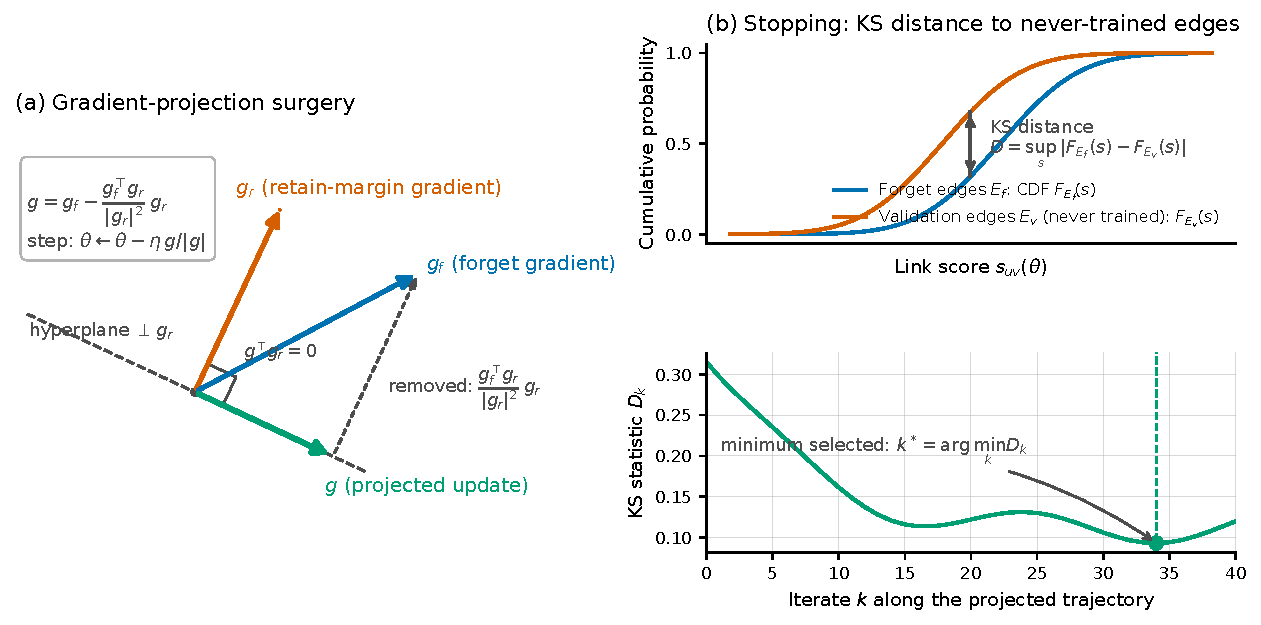
\includegraphics[width=0.92\textwidth]{Fig1.pdf}\caption{(a) The forget gradient $g_f$ is projected onto the hyperplane orthogonal to the retain-margin gradient $g_r$; the update $g$ lowers forget-edge scores without harming the margin to first order. (b) Stopping selects the iterate whose forget-edge score distribution is least distinguishable (two-sample KS) from never-trained validation edges.}\end{figure}

\textbf{Retain-margin anchor.} The direction that raises the retained link-prediction margin is
\begin{equation}
g_r = \nabla_\theta \left[ \frac{1}{|E_r|} \sum_{(u,v)\in E_r} s_{uv}(\theta) - \frac{1}{|N_r|} \sum_{(u,v)\in N_r} s_{uv}(\theta) \right],
\end{equation}
again under $A_r$. Unlike a classification loss on retained nodes, this margin is the exact quantity link-prediction utility depends on; unlike a minibatch estimate, it uses the complete retained edge set with an equal-sized non-edge set, making it a deterministic anchor with no subsampling noise.

\subsection{Surgery and normalized descent}
The surgically corrected update removes from the forget direction any component that would harm the retain margin:
\begin{equation}
g = g_f - \frac{g_f^\top g_r}{\|g_r\|^2} g_r, \qquad \theta \leftarrow \theta - \eta \frac{g}{\|g\|},
\end{equation}
with step size $\eta = 0.05$ in our experiments. By construction $g^\top g_r = 0$: to first order, each step leaves the retain margin unchanged while decreasing the mean forget-edge logit. This is precisely the failure mode of naive gradient ascent (NegGrad), which descends along $g_f$ unprojected and therefore erodes $E_r$ utility whenever $g_f$ and $g_r$ conflict---the typical case on real graphs.

\subsection{First-order analysis}
Let $M(\theta) = \frac{1}{|E_r|}\sum_{E_r} s_{uv} - \frac{1}{|N_r|}\sum_{N_r} s_{uv}$ be the retain margin, so that $g_r = \nabla M(\theta)$, and let $F(\theta) = \frac{1}{|E_f|}\sum_{E_f} s_{uv}$ be the mean forget-edge logit, so that $g_f = \nabla F(\theta)$.

\textbf{Proposition 1.} For the update (3) with $\eta > 0$ small, and assuming $g \neq 0$: (i) the retain margin is stationary to first order, $M(\theta - \eta g/\|g\|) = M(\theta) + o(\eta)$; (ii) the mean forget-edge logit strictly decreases to first order, $F(\theta - \eta g/\|g\|) = F(\theta) - \eta\|g\| + o(\eta)$; (iii) $g_f^\top g = \|g\|^2 \geq 0$, with equality only if $g_f$ is parallel (or anti-parallel) to $g_r$.

\textbf{Proof.} (i) By Taylor expansion, $M(\theta - \eta g/\|g\|) = M(\theta) - \eta \nabla M(\theta)^\top g/\|g\| + o(\eta)$, and $\nabla M(\theta)^\top g = g_r^\top g = 0$ by construction of the projection. (ii) is the same expansion applied to $F$. (iii) follows from $g_f^\top g = g_f^\top g_f - (g_f^\top g_r)^2/\|g_r\|^2 = \|g_f\|^2 - \|P_{g_r} g_f\|^2 = \|g_f - P_{g_r} g_f\|^2 = \|g\|^2$, where $P_{g_r}$ is the orthogonal projector onto $g_r$. $\square$

The proposition is worth reading for what it does and does not promise. Part (i) is the precise sense in which the surgery protects utility: no first-order harm to the retain margin, unlike NegGrad. The argument is a special case of the general retain-invariance theorem of Zhou et al.\ \cite{gu2025}, who prove that a small update leaves the retain loss invariant if and only if it is orthogonal to the subspace spanned by retain gradients; we credit that result and claim only its application to the link-prediction margin. Part (iii) shows the forget direction is never reversed by the projection ($g_f^\top g \geq 0$), so forgetting proceeds monotonically to first order---except in the degenerate case where $g_f$ is parallel (or anti-parallel) to $g_r$, i.e., forgetting the deleted edges and preserving the margin are the same direction, in which case $g = 0$ and the normalized step is undefined (in practice we skip the update). The analysis is first-order and local, and its ``small $\eta$'' premise is asserted rather than checked (no $\eta$ sensitivity is reported): over many steps the anchor $g_r$ itself moves, which is why the empirical trajectory---not the single-step calculation---is what Section 6 evaluates. This is a local calculation, not an unlearning guarantee: it says nothing about how far the trajectory can travel before the anchor moves, which is exactly what breaks at 20\% deletion on Cora (Section 6.2).

\subsection{Calibrated stopping rules}
A fixed iteration budget is a per-dataset hyperparameter in disguise. FGS instead runs a projected trajectory and keeps one iterate selected by a data-driven rule computed on validation edges, which were never trained on and are absent from $A_r$---the same informational position forgotten edges occupy under retraining. Validation edges are a proxy, not a perfect stand-in: the base model was trained on the same graph, so validation-edge endpoints carry structural signal a retrained model never sees (cf.\ Remark 1). The KS rule therefore targets distributional similarity under this proxy; Section 6.4 shows where the proxy diverges from the attack optimum. We use only validation data; attack negatives and test edges are never touched during unlearning: $E_v$ is disjoint from the test split and from the evaluation hard-negative set. We test five variants, summarized in Table 3:

\begin{table}[htbp]\centering\small
\caption{The five variants at a glance: three stopping rules for the projected run and the two no-projection ablations. ``Cost'' is the stopping overhead beyond the shared trajectory. The margin-guarded KS variant of Section 4.4 is a negative result reported in the text; it is not a headline variant and is not listed here.}
\begin{tabular}{p{3.2cm}p{5.5cm}p{3.5cm}}\toprule Variant & Selection rule & Cost\\\midrule
fgs (KS) & iterate minimizing KS(forget scores, validation scores) & 40-step trajectory\\
fgs attack (attack-calibrated) & iterate minimizing $|\mathrm{AUC}(\mathrm{forget\ vs\ stop\text{-}neg}) - \mathrm{AUC}(\mathrm{validation\ vs\ stop\text{-}neg})|$ & 80-step trajectory + scoring\\
fgs hybrid (hybrid) & attack-calibrated key on the five lowest-KS iterates & 40-step trajectory + 5 scorings\\
fgs noproj-attack (no-proj., attack stop) & attack-calibrated stopping with the projection removed ($g = g_f$) & 80-step trajectory + scoring\\
fgs noproj-KS (no-proj., KS stop) & KS stopping with the projection removed ($g = g_f$) & 40-step trajectory\\\bottomrule
\end{tabular}\end{table}

Every variant runs its trajectory to the full step budget and scores every iterate as it is produced; the stopping rule selects from the completed trajectory, retrospectively, and never terminates the run early. ``Stopping'' in this paper therefore names checkpoint selection over a fixed candidate set, not a computation saving.

\textbf{KS rule (fgs).} Run up to $T_{max} = 40$ projected steps; keep the iterate minimizing the two-sample Kolmogorov--Smirnov statistic \cite{massey1951} between the forgotten-edge scores and the validation-edge scores. The KS minimum is a heuristic proxy for ``looks retrained'': if the forgotten-edge scores were drawn from the same distribution as the validation-edge scores, a membership-style adversary could not distinguish them. We use the KS statistic rather than a mean gap because indistinguishability is a distributional property: means can match while variances differ, leaving the adversary signal. Matching the retrain gap under this fixed auditor is an empirical indistinguishability claim, not a privacy guarantee: a stronger or adaptive auditor could still tell the unlearned model apart from retraining.

\textbf{Margin-guarded KS (fgs margin).} A tried fix for early KS alignment: restrict the KS minimization to iterates satisfying $\mathrm{mean}_{E_f} s \leq \mathrm{mean}_{E_v} s$, falling back to the maximum-forgetting iterate if none qualify. This is a non-dataset-specific rule: no threshold is tuned, only the inequality direction is fixed. It fails---the guard essentially never binds, and the variant is statistically identical to plain KS (Section 6). We keep it as a negative result.

\textbf{Attack-calibrated rule (fgs attack).} Run up to 80 projected steps; keep the iterate minimizing $|\mathrm{AUC}(\mathrm{forget\ vs\ held\text{-}out\ stop\ negatives}) - \mathrm{AUC}(\mathrm{validation\ vs\ held\text{-}out\ stop\ negatives})|$, where the stop negatives are freshly sampled hard negatives disjoint from the evaluation attack negatives. This directly calibrates the forget-vs-nonedge ranking---what the membership-inference-style attack measures \cite{shokri2017}---to the unseen-edge ranking. It explicitly targets attack-style ranking and should be read as such: a validation-calibrated rule, not a test-set-tuned one, and not a purely unsupervised stopping rule. It removes the speed advantage (all 80 candidates are evaluated) but substantially closes the CiteSeer attack gap (Section 6). (The related shadow-retrain stop of Limitation 5 sits on a flat KS curve and is unstable per seed; re-computation from the archived trajectories brackets its reported gap at +0.051 to +0.060, with the paired difference significant in both computations and the conclusion unchanged.)

\begin{figure}[htbp]\centering\fbox{\parbox{0.92\textwidth}{\textbf{Algorithm 1: Forget Gradient Surgery (FGS)}\\ Input: trained $\theta$, post-deletion adjacency $A_r$, forget edges $E_f$, retained edges $E_r$, non-edges $N_r$, validation edges $E_v$, budget $T_{max}$, step size $\eta$\\ Output: unlearned parameters $\theta_{k^\star}$\\ $\theta_0 \leftarrow \theta$; $d_0 \leftarrow \mathrm{KS}(\{s_{uv}(\theta_0)\}_{E_f}, \{s_{uv}(\theta_0)\}_{E_v})$; $k^\star \leftarrow 0$; $d^\star \leftarrow d_0$\\ for $t = 1$ to $T_{max}$ do: compute $g_f$ by (1) and $g_r$ by (2) under $A_r$; $g \leftarrow g_f - (g_f^\top g_r/\|g_r\|^2) g_r$; $\theta_t \leftarrow \theta_{t-1} - \eta g/\|g\|$; $d_t \leftarrow \mathrm{KS}(\{s_{uv}(\theta_t)\}_{E_f}, \{s_{uv}(\theta_t)\}_{E_v})$; if $d_t < d^\star$ then $d^\star \leftarrow d_t$; $k^\star \leftarrow t$; end for; return $\theta_{k^\star}$}}
\caption{Forget Gradient Surgery with KS stopping. The iterate-0 evaluation ($d_0$, $k^\star \leftarrow 0$) is essential, not incidental: the implementation scores the post-deletion model before any gradient step, and the KS minimum can occur there (e.g., PubMed seed 7), in which case FGS returns the model unchanged.}
\end{figure}

\textbf{Hybrid rule (fgs hybrid).} A lower-cost attack-calibrated variant: run the 40-step KS trajectory, keep the five iterates with the lowest KS values, and apply the attack-calibrated key to those five only. This preserves the ranking calibration where the KS proxy is weakest while avoiding the 80-candidate evaluation cost of fgs attack.

\subsection{Complexity}
Each step performs one forward pass and two backward passes (one for $g_f$, one for $g_r$) over $|E_f| + |E_r| + |N_r|$ scored pairs; with $|E_f| \ll |E_r|$ this is $O(T_{max} \cdot (|E_r| + |N_r|))$ score evaluations and no Hessian, no sharding, no added parameters, and no retraining. We report wall-clock cost in Section 6.

\section{Experimental Setup}
\textbf{Datasets and task.} We use Cora, CiteSeer, and PubMed \cite{planetoid2016} with the standard link-prediction split: edges are divided 70/15/15 into train / validation / test; the train split is further divided into a forget set $E_f$ (a random fraction $p$ of train edges) and a retained set $E_r$. Validation edges $E_v$ are never trained on and never part of $A_r$. Backbone: a two-layer GCN (32-dimensional hidden layer, ReLU) trained with Adam ($10^{-2}$, 150 epochs, full batch) on link prediction with dot-product logits. All base models use identical initializations and data splits for every method.

\textbf{Methods.} Retrain (gold standard), Fine-tune (extra training on $(X, A_r)$), NegGrad (gradient ascent on $E_f$), GNNDelete---our adaptation of GNNDelete, a NumPy port of the deletion-operator method of Cheng et al.\ \cite{gnndelete2023} to edge unlearning (trainable per-layer linear operators on the forget-edge endpoints, trained for 40 epochs with a deleted-edge-consistency loss toward the non-edge class plus a neighborhood-influence loss matching the base model's scores). Its five deviations from Cheng et al.\ are: D1, the affected region is the forget-edge endpoints (1-hop); D2, the deleted-edge-consistency loss is adapted to binary cross-entropy toward the non-edge class on link scores (the binary analogue of KL-to-uniform); D3, the neighborhood-influence loss is adapted to mean-squared error against base-model link scores; D4, NumPy instead of PyTorch/PyG, on this harness's own link-prediction base model; D5, per-layer identity-initialized linear operators trained 40 epochs at learning rate 0.01. The port remains an adaptation, not the official implementation, and its validation status is stated per dataset, under the rule that a reimplementation used as a run baseline is validated against the original's published numbers or labelled unvalidated. On Cheng et al.'s own AUROC($E_d$) statistic (port minus retrain at $\lambda = 1.0$), the port's PubMed deltas are $+0.202$ on each of three seeds (mean $+0.202$), inside the published range ($+0.188$ to $+0.240$), and its utility retention sits in the published regime: the port is \textbf{validated} on PubMed. On Cora the same statistic lands at the retrain level ($\Delta = -0.023$, two seeds) rather than at the published separation, for an identified protocol reason (the FGS retrain reference already separates deleted from remaining edges at 0.750, leaving little headroom for the statistic to register): the port is \textbf{unvalidated} on Cora. CiteSeer is \textbf{unvalidated} because it is not among Cheng et al.'s datasets, so no published number exists to validate against. Absolute AUROC levels are not used for validation on any dataset, since they measure the base model and split rather than the unlearning method. The neighborhood-influence weight $\lambda$ is tuned per dataset on five held-out tuning seeds (1001, 2002, 3003, 4004, 5005) disjoint from every evaluation seed, over the grid $\{0.25, 0.5, 1, 2, 4\}$, by a rule frozen before tuning ran: the smallest mean $|\Delta_{atk}|$ among $\lambda$ with mean utility gap $\geq -0.02$, ties to the smaller $\lambda$. The selected weights are $\lambda^\star = 1.0$ (Cora), $0.5$ (CiteSeer), and $4.0$ (PubMed). Table 4 keeps the fixed $\lambda = 1.0$ port setting for comparability with the other untuned baselines; the tuned head-to-head is Table 5. Documented in the reproduction package---and UtU, the unlink-only baseline: the base model (trained with the forget edges) evaluated on the post-deletion adjacency $A_r$, with no parameter change. Then FGS with the stopping variants of Section 4.4: fgs (KS), fgs margin (margin-guarded KS), fgs attack (attack-calibrated), fgs hybrid (hybrid, CiteSeer only), and two no-projection ablations that run the identical code path with the projection removed ($g = g_f$): fgs noproj-attack, with the same attack-calibrated stopping as fgs attack, and fgs noproj-KS, with the same KS stopping as fgs---so each projected/unprojected pair, differing only in the projection, tests the surgery's contribution under its stopping rule. The KS-stopped pair is the cleaner of the two tests, because it is free of the auditor circularity of Limitation 5.

\textbf{MEGU baseline.} MEGU \cite{megu2024} is run from its official code (github.com/xkLi-Allen/MEGU, commit 03bbb358) with its unlearning loop unmodified and its published hyperparameters, untuned. The protocol mapping substitutes exactly the FGS forget set at 5\% of train edges for the method's default deletion request, and link scores are computed from the encoder embeddings with a dot-product decoder. \textbf{ETR baseline.} ETR \cite{etr2024} is run from its official code (github.com/AllminerLab/ETR, commit c88ec74) with its published-default hyperparameters, untuned, under the same protocol mapping: exactly the FGS forget set at 5\%, with link scores from the penultimate-layer embeddings over the remain graph. \textbf{Governing caveat for both baselines.} Both methods' encoders are node classifiers never trained on edges, so their absolute AUCs are not like-for-like with the link-prediction baselines, and their gaps against the FGS retrain reference conflate unlearning behavior with classifier-embeddings-as-link-features. Their gaps are per-seed paired differences against the harness's retrain-from-scratch reference for the same seed---the identical reference underlying every other row of Table 4 (retrain attack AUC means 0.703/0.768/0.917; utility means 0.774/0.794/0.939)---read from the harness's per-seed outputs; neither adapter ran nor referenced its own retrain. This caveat governs every use of the MEGU and ETR rows below.

\textbf{Metrics.} Forgetting: attack AUC (link-inference separating $E_f$ from hard non-edges), reported as the gap to retrain, $\Delta_{atk} = \mathrm{AUC}_{atk}(\theta_u) - \mathrm{AUC}_{atk}(\theta_{re})$; zero means indistinguishable from retraining. The sign is read in words: a positive attack gap means the unlearned model is more vulnerable than retrain (under-forgetting); a negative gap means it is less vulnerable (over-forgetting). Utility: test-set link AUC, reported as the signed gap to retrain, $\Delta_{util} = \mathrm{AUC}_{util}(\theta_u) - \mathrm{AUC}_{util}(\theta_{re})$ (retrain test AUC is 0.774/0.794/0.939 on Cora/CiteSeer/PubMed, so the gap is the meaningful quantity). Because the attack negatives are label-matched (Section 3), the auditor is stronger in that one respect than a label-blind adversary; the asymmetry is identical for the unlearned and retrained models, so it cancels in the gap, and every gap below is read as auditor-relative---indistinguishability under this auditor---rather than as an absolute privacy level. \textbf{Predeclared head-to-head criterion.} The primary criterion for every head-to-head comparison in this paper, stated here before any comparison is reported, is the absolute attack gap $|\Delta_{atk}|$ to retraining---smaller is closer to retraining---with paired tests computed on per-seed absolute gaps. Signed gaps are reported for direction only (under- versus over-forgetting) and are never the basis of a comparative claim. Efficiency: wall-clock time relative to retraining on identical hardware (2 CPUs, no GPU).

\textbf{Protocol.} Main sweep: 5\% forget fraction on three datasets $\times$ ten seeds (42, 7, 123, 2024, 31337, 999, 2025, 5555, 7777, 31338). Fraction sensitivity: 1\%, 10\%, 20\% on five seeds (42, 123, 2024, 2025, 999)---a fixed subset of the ten main seeds, held constant across all fractions. Randomness: seed controls initialization, the forget-set draw, and the retain-non-edge draw $N_r$. Retrain uses the same seed. Statistics: paired (within-seed) comparisons with paired two-sided t-tests; $d_z$ is Cohen's paired effect size. Retrospectively, with $n = 10$ paired seeds, the design detects Cohen's paired $d_z \approx 1.0$ at 80\% power ($\alpha = 0.05$, two-sided); the decisive headline effects exceed this bar, while the marginal untuned FGS-vs-GNNDelete gaps ($d_z \approx -0.75$) fall below it and are reported as directional only. All reported means are $\pm$ one standard deviation across seeds. For the $n = 5$ fraction-sensitivity comparisons, where skew is a concern, we also report Wilcoxon signed-rank p-values; at $n = 5$ the two-sided Wilcoxon signed-rank test cannot return $p$ below 0.0625, so the fraction-sweep tests are descriptive. Paired Wilcoxon signed-rank tests, where reported alongside the t-tests, are likewise reported unadjusted across the study's comparisons. Multiplicity is handled for the headline family: the 15 headline paired tests (the Table 4 attack and utility gaps to retrain for fine-tune, NegGrad, GNNDelete at $\lambda = 1.0$, and UtU; the $\lambda = 1.0$ FGS--GNNDelete head-to-heads; and the CiteSeer FGS attack gap) are corrected as one family by the Benjamini--Hochberg procedure. Fourteen of the 15 survive at $q < 0.05$; the single failure---the CiteSeer FGS attack gap vs.\ retrain, raw $p = 0.094$---was never significant before correction either. Nine of the 15 survive Bonferroni. Findings that survive Benjamini--Hochberg but not Bonferroni (the $\lambda = 1.0$ GNNDelete attack gaps on Cora and CiteSeer, the PubMed fine-tune attack gap, and the two $\lambda = 1.0$ head-to-heads) are worded as BH-only wherever they are stated. The Section 6.1 tests (tuned head-to-head, KS-stopped ablation, TOST) are reported with raw paired p-values and read under the band rule below. Equivalence is tested rather than inferred from non-significance: for the headline FGS attack gaps we run two one-sided tests (TOST) at the pre-stated $\pm 0.02$ AUC margin of Section 6.1, reporting the smallest margin each dataset supports and the power at the stated margin. We flag the $n = 5$ exploratory comparisons as such rather than leaning on uncorrected p-values. Throughout, any $p$ between 0.01 and 0.05 outside the corrected headline family is treated as exploratory evidence only; no load-bearing claim rests on an uncorrected value in that band alone.

\textbf{Threats to validity and scope.} (i) The auditor is fixed and non-adaptive; stronger adaptive attackers (e.g., shadow models) could find residual signal we cannot see. One related check---a per-seed shadow-retrain stopping check, in which the auditor and its scoring are unchanged and only the stopping calibration changes---is tested in Section 8. We make no certified-unlearning claim. (ii) We scope to edge deletion on homophilic citation graphs with a GCN; node and feature deletion are out of scope. (iii) Absolute attack AUC stays high even after retraining (Remark 1); our metric is the retrain gap, which is the correct target but means ``forgotten'' does not mean ``unpredictable.'' (iv) FGS touches only the parameters, not the adjacency: structural deletion (Unlink) is a separate, complementary step. (v) One GraphSAGE transfer configuration is reported; it is a smoke test, not generalization evidence.

\textbf{AI use.} The author used the AI tool Muse (Muse Spark 1.3, Meta) for drafting and grammatical editing. The contents are reviewed, edited, and attested for accuracy by the author.

\section{Results}
\subsection{Main comparison: 5\% deletion, ten seeds}
At 5\% deletion, FGS with KS stopping (fgs) is at or tied-closest to retraining among the approximate methods on Cora and PubMed, and tied with the tuned GNNDelete port on CiteSeer (Table 4; the tuned comparison is Table 5). Table 4 reports attack and utility gaps to retrain with paired statistics ($n = 10$ seeds). The 95\% CIs (paired) for the KS-stopped FGS attack gaps are $[-0.005, +0.020]$ on Cora, $[-0.008, +0.081]$ on CiteSeer, and $[-0.003, +0.006]$ on PubMed. We read these against a $\pm 0.02$ AUC equivalence margin: 0.02 is about 2\% of the retrain attack-AUC scale ($\approx 0.9$) and sits well below the gaps that mark genuine failures in this study (fine-tuning leaves +0.09--+0.12; NegGrad costs $-0.06$--$-0.09$ utility), so containment under it is a demanding bar. Against this margin, only PubMed's interval is fully contained, Cora's straddles the margin's upper edge, and CiteSeer's lies outside it on the high side. The margin itself is author-chosen, so the Cora containment reading is margin-sensitive rather than absolute. We now test equivalence formally at that margin (two one-sided tests on the per-seed gaps, $\alpha = 0.05$). PubMed is equivalent to retraining at $\pm$0.02 (TOST $p < 0.001$; the data support a margin as tight as $\pm$0.0049, and power at the stated margin exceeds 0.99). Cora is also equivalent at $\pm$0.02 (TOST $p = 0.027$; smallest supported margin $\pm$0.0179; power 0.89 if the true gap were zero and 0.64 at the observed mean). CiteSeer is not equivalent (TOST $p = 0.79$; smallest supported margin $\pm$0.0728), and at its observed variance, equivalence at $\pm$0.02 with 80\% power would require $\approx$85 seeds---an order of magnitude beyond this study---so CiteSeer equivalence is an open negative, not a null that a feasible extension of this design would resolve. Non-significance alone is still never read as equivalence anywhere else in this paper: the design detects only large paired effects ($d_z \approx 1.0$ at 80\% power; Section 5). On CiteSeer, the FGS attack gap is not significant at $n = 10$ (paired vs.\ retrain $p = 0.09$, $d_z = 0.59$), and the mean is driven substantially by a single outlier seed (+0.181; dropping it moves the mean to +0.021; see Section 7 for the leave-one-out robustness analysis); the per-seed median attack gap on CiteSeer is +0.018, against the mean of +0.037.

Three patterns held up across the sweep:

\textbf{1. Fine-tuning does not forget; ascent destroys utility.} Fine-tuning on the retained graph leaves large attack gaps: +0.090 on Cora and +0.116 on CiteSeer (both $p < 0.001$, $d_z = 3.69/2.17$), confirming that residual parametric memory of the deleted edges survives additional training. NegGrad reduces the attack gap but at a steep utility cost: $-0.085$ on Cora, $-0.079$ on CiteSeer, $-0.062$ on PubMed (all $p < 0.001$, $|d_z| > 2.4$), consistent with the blast-radius analysis---unprojected ascent on $E_f$ backpropagates through the receptive fields of retained edges. The GNNDelete deletion-operator baseline (our NumPy port; validation status per dataset in Section 5---validated on PubMed, unvalidated on Cora and CiteSeer) sits between the two at its untuned $\lambda = 1.0$ setting: on Cora its attack gap is +0.022 ($p = 0.011$, $d_z = 1.01$) and on CiteSeer +0.052 ($p = 0.015$, $d_z = 0.95$)---materially better than fine-tuning but roughly 2--3$\times$ the FGS gap---while on PubMed it over-forgets severely (attack gap $-0.085$, $p < 0.001$, $d_z = -14.2$), pushing forget-edge scores well below the retrain reference. Both $\lambda = 1.0$ attack gaps survive Benjamini--Hochberg correction within the headline family but not Bonferroni, and are read as BH-only. Unlinking alone (UtU) is not enough: attack gaps of +0.058 on Cora and +0.105 on CiteSeer (both $p < 0.001$, $d_z = 2.72/1.94$) confirm the blast-radius hypothesis---the parameters' residual memory of the deleted edges survives structural deletion. (On PubMed the unlink-only gap is just +0.009, so structural deletion does most of the work there.) Paired head-to-head at $\lambda = 1.0$ (same seeds, signed FGS$-$GNNDelete attack-gap difference), the signed difference favors FGS on Cora ($-0.014$, $p = 0.034$, $d_z = -0.79$, 95\% CI $[-0.027, -0.001]$) and CiteSeer ($-0.015$, $p = 0.044$, $d_z = -0.74$, 95\% CI $[-0.030, -0.001]$), while on PubMed the signed difference is positive (+0.087, $p < 0.001$, $d_z = +10.9$, 95\% CI $[+0.081, +0.093]$) because GNNDelete over-forgets. The Cora and CiteSeer signed differences are marginal and survive Benjamini--Hochberg but not Bonferroni within the headline family---BH-only, directional evidence. Read under the predeclared primary criterion (absolute attack gap, Section 5), the $\lambda = 1.0$ means order the same way on Cora ($|\Delta_{atk}|$ 0.008 vs.\ 0.022) and CiteSeer (0.037 vs.\ 0.052), and on PubMed the baseline's signed gap is over-forgetting, so the absolute reading favors FGS there as well (0.002 vs.\ 0.085). The tuned comparison below is the primary head-to-head.

\begin{table}[htbp]\centering\tiny\setlength{\tabcolsep}{2.5pt}
\caption{5\% deletion, ten seeds per dataset: attack gap $\Delta_{atk}$ and utility gap $\Delta_{util}$ to retrain (mean$\pm$SD; 0 = identical to retrain), with paired two-sided t-test p-values vs.\ retrain. On each dataset, seeds 7, 42, 123 come from an earlier run and the other seven from a later run under the same protocol. Exchangeability is established by re-running the three earlier seeds per dataset under the frozen pipeline: every method's attack/util reproduces within $3 \times 10^{-3}$ (floating-point noise), confirming identical code paths, splits, and hyperparameters. All comparisons are within-seed paired. Sign guide: $\Delta_{atk} > 0$ means the unlearned model is more vulnerable than retrain (under-forgetting, worse); $\Delta_{atk} < 0$ means less vulnerable (over-forgetting); $\Delta_{util} < 0$ is a utility loss (worse). The fgs hybrid row reports the CiteSeer attack gap only (mean +0.027 over the same ten seeds; per-seed values in Table 6); the hybrid was evaluated on CiteSeer alone. The MEGU and ETR rows report mean$\pm$SD only (no paired p-values were computed for them) and carry the base-model caveat of Section 5: both methods' encoders are node classifiers never trained on edges, so their absolute AUCs are not like-for-like with the link-prediction baselines. The MEGU and ETR gaps are per-seed paired differences against the same harness retrain-from-scratch reference as every other row of this table---retrain attack AUC means 0.703/0.768/0.917 and utility means 0.774/0.794/0.939 on Cora/CiteSeer/PubMed, read from the harness's per-seed outputs; no adapter-side retrain was used. For KS-stopped FGS on CiteSeer, the per-seed median attack gap is +0.018 (mean +0.037).}
\begin{tabular}{lcccccc}\toprule & \multicolumn{2}{c}{Cora} & \multicolumn{2}{c}{CiteSeer} & \multicolumn{2}{c}{PubMed}\\
Method & $\Delta_{atk}$ & $\Delta_{util}$ & $\Delta_{atk}$ & $\Delta_{util}$ & $\Delta_{atk}$ & $\Delta_{util}$\\\midrule
Fine-tune & +0.090$\pm$0.024 & $-0.013$$\pm$0.023 & +0.116$\pm$0.053 & $-0.001$$\pm$0.026 & +0.003$\pm$0.003 & $-0.003$$\pm$0.002\\
NegGrad & +0.012$\pm$0.054 & $-0.085$$\pm$0.025 & +0.005$\pm$0.058 & $-0.079$$\pm$0.032 & $-0.068$$\pm$0.014 & $-0.062$$\pm$0.017\\
GNNDelete & +0.022$\pm$0.022 & $-0.017$$\pm$0.022 & +0.052$\pm$0.055 & $-0.004$$\pm$0.021 & $-0.085$$\pm$0.006 & $-0.007$$\pm$0.002\\
UtU & +0.058$\pm$0.021 & $-0.015$$\pm$0.023 & +0.105$\pm$0.054 & $-0.003$$\pm$0.022 & +0.009$\pm$0.004 & +0.004$\pm$0.002\\
fgs (KS) & +0.008$\pm$0.017 & $-0.020$$\pm$0.023 & +0.037$\pm$0.062 & $-0.011$$\pm$0.023 & +0.002$\pm$0.006 & $-0.000$$\pm$0.004\\
fgs margin & +0.008$\pm$0.019 & $-0.020$$\pm$0.023 & +0.037$\pm$0.062 & $-0.011$$\pm$0.023 & +0.000$\pm$0.006 & $-0.001$$\pm$0.004\\
fgs attack & +0.001$\pm$0.020 & $-0.022$$\pm$0.023 & +0.008$\pm$0.070 & $-0.017$$\pm$0.023 & $-0.017$$\pm$0.013 & $-0.012$$\pm$0.009\\
fgs hybrid & --- & --- & +0.027 (attack only) & see caption & --- & ---\\
fgs noproj-attack & $-0.014$$\pm$0.026 & $-0.048$$\pm$0.019 & $-0.011$$\pm$0.072 & $-0.053$$\pm$0.019 & $-0.010$$\pm$0.031 & $-0.014$$\pm$0.025\\
\midrule
\multicolumn{7}{l}{\textit{Descriptive only (disclosed encoder caveat, Section 5):}}\\
MEGU & $-0.103$$\pm$0.028 & +0.043$\pm$0.022 & $-0.129$$\pm$0.057 & +0.031$\pm$0.015 & $-0.132$$\pm$0.013 & $-0.078$$\pm$0.010\\
ETR & $-0.027$$\pm$0.046 & +0.017$\pm$0.027 & $-0.093$$\pm$0.062 & $-0.000$$\pm$0.023 & $-0.045$$\pm$0.005 & $-0.020$$\pm$0.004\\\bottomrule
\end{tabular}\end{table}

\textbf{GNNDelete held-out tuning and the tuned head-to-head.} The $\lambda = 1.0$ rows above are one point on a deletion-vs-neighborhood tradeoff, taken untuned. The tradeoff weight is tuned on five held-out tuning seeds disjoint from the evaluation seeds, by the frozen rule of Section 5, giving $\lambda^\star = 1.0$ (Cora), $0.5$ (CiteSeer), and $4.0$ (PubMed); tuning never touches the evaluation seeds, since selecting on them would inflate the selected point. At $\lambda^\star$ the tuned port's attack gaps are +0.022 $\pm$ 0.022 on Cora (unchanged---$\lambda^\star$ is the Table 4 setting there), +0.010 $\pm$ 0.058 on CiteSeer, and $-0.014$ $\pm$ 0.004 on PubMed: held-out tuning removes the severe PubMed over-forget ($-0.085 \to -0.014$) that the untuned row suggested, confirming that it was a port-setting artifact. The tuned head-to-head (Table 5) compares absolute attack gaps, the predeclared primary criterion of Section 5. FGS's $|\Delta_{atk}|$ is smaller on PubMed by 0.010 (paired $p < 0.001$, $d_z = -2.38$) and on Cora by 0.012 (paired $p = 0.037$, $d_z = -0.78$; in the marginal band of Section 5, read as directional-plus rather than decisive). On CiteSeer the absolute gaps tie (difference +0.005, $p = 0.56$), while the signed comparison favors the tuned baseline (FGS $-$ tuned GNNDelete $= +0.027$, $p = 0.0095$, $d_z = 1.04$): CiteSeer is FGS's weakest dataset under every reading in this study. The tuned baseline's utility gaps ($-0.017$ on Cora, $-0.005$ on CiteSeer, $+0.002$ on PubMed) are comparable to FGS's, and it remains the faster procedure (Section 6.3).

\begin{table}[htbp]\centering\scriptsize\setlength{\tabcolsep}{3pt}
\caption{Tuned head-to-head at 5\% deletion, ten evaluation seeds. $\lambda^\star$ was selected on five held-out tuning seeds by the frozen rule of Section 5 (grid $\{0.25, 0.5, 1, 2, 4\}$), never on these seeds. Attack and utility gaps are mean$\pm$SD against the same retrain reference as Table 4. The $|\Delta_{atk}|$ difference is the paired per-seed difference of absolute attack gaps (FGS minus tuned GNNDelete) with its paired two-sided p-value; negative means FGS is closer to retraining. The signed CiteSeer difference ($+0.027$, $p = 0.0095$) favors the tuned baseline; see the text.}
\begin{tabular}{lccccc}\toprule & $\lambda^\star$ & GNNDelete (tuned) $\Delta_{atk}$ & FGS $\Delta_{atk}$ & GNNDelete (tuned) $\Delta_{util}$ & $|\Delta_{atk}|$ diff.\ ($p$)\\\midrule
Cora & 1.0 & +0.022$\pm$0.022 & +0.008$\pm$0.017 & $-0.017$$\pm$0.022 & $-0.012$ (0.037)\\
CiteSeer & 0.5 & +0.010$\pm$0.058 & +0.037$\pm$0.062 & $-0.005$$\pm$0.021 & +0.005 (0.56)\\
PubMed & 4.0 & $-0.014$$\pm$0.004 & +0.002$\pm$0.006 & +0.002$\pm$0.002 & $-0.010$ ($<0.001$)\\\bottomrule
\end{tabular}\end{table}

\textbf{MEGU head-to-head.} MEGU over-forgets on all three datasets (reported descriptively only, and subject to the embedding-geometry artifact reading stated below): its attack gap is negative on 30/30 seeds (Cora $-0.103$ $\pm$ 0.028; CiteSeer $-0.129$ $\pm$ 0.057; PubMed $-0.132$ $\pm$ 0.013)---the same failure direction as the GNNDelete port on PubMed---driving forget-edge scores consistently below the retrain reference. Its utility sits above the retrain reference on Cora (+0.043) and CiteSeer (+0.031) but below it on PubMed ($-0.078$), at median time ratios of 0.068/0.052/0.045 (Section 6.3).

\textbf{ETR head-to-head.} ETR also over-forgets on average on all three datasets (reported descriptively only, and subject to the same artifact reading) (Cora $-0.027$ $\pm$ 0.046; CiteSeer $-0.093$ $\pm$ 0.062; PubMed $-0.045$ $\pm$ 0.005), negative on 26/30 seeds and smaller in magnitude than MEGU on every dataset. Its utility is essentially at the retrain reference on CiteSeer ($-0.000$), above it on Cora (+0.017), and below it on PubMed ($-0.020$), and it is the fastest procedure of all methods run (Section 6.3). For MEGU, the pattern itself---attack gap well below retrain with utility above it on two datasets---is also consistent with an embedding-geometry artifact of scoring links from classifier embeddings, which is why these rows are reported descriptively only (Table 4, below the rule) and no comparative conclusion is drawn from them.

\textbf{2. The projection preserves utility---under both stopping rules---and it does not forget.} The no-projection ablation fgs noproj-attack runs the identical code path with the projection removed ($g = g_f$) and the same attack-calibrated stopping as fgs attack, so the paired fgs attack $-$ fgs noproj-attack comparison isolates the projection under that stopping rule: the only difference between the two runs is the orthogonal projection. The projected variant preserves substantially more utility: the paired utility difference is +0.027 on Cora ($p < 0.001$, $d_z = 2.95$) and +0.036 on CiteSeer ($p < 0.001$, $d_z = 4.29$); on PubMed, there is no detectable difference (+0.002, $p = 0.83$), where even the unprojected run preserves utility. Against retrain, the no-projection variant sits $-0.048$ lower on Cora and $-0.053$ on CiteSeer (Table 4). Forgetting is comparable with or without the projection (paired attack differences +0.015 to +0.019 on Cora/CiteSeer), but the utility cost of the unprojected run is unacceptable---exactly the tradeoff the method is designed to avoid. That ablation uses the attack-calibrated stopping rule, which the Limitations (Section 8) show is auditor-circular, so on its own it would demonstrate the projection's benefit only under that rule. The cleaner test is the KS-stopped pair: fgs noproj-KS is the identical code path with the projection removed and the same KS stopping as fgs. Its attack gaps to retrain are $-0.002$ $\pm$ 0.017 on Cora ($p = 0.75$), $+0.028$ $\pm$ 0.064 on CiteSeer ($p = 0.20$), and $+0.005$ $\pm$ 0.010 on PubMed ($p = 0.19$)---no detectable difference from retraining on any dataset, so under KS stopping the unprojected ascent already forgets to the retrain level, and the projection is not the forgetting mechanism. (The projected run's gaps under the same rule are Table 4's fgs row; the paired projected-minus-unprojected attack differences are +0.011 on Cora ($p = 0.007$), +0.007 on CiteSeer ($p = 0.32$), and $-0.004$ on PubMed ($p = 0.14$)---small, and on Cora in the direction of the unprojected run sitting closer to retrain.) What the projection changes is utility: the paired utility difference (projected minus unprojected) is +0.023 on Cora ($p < 0.001$, $d_z = 3.14$) and +0.030 on CiteSeer ($p < 0.001$, $d_z = 3.88$), and +0.000 on PubMed ($p = 0.93$), where the unprojected run loses nothing to begin with (its utility gap is $-0.001$). Against retrain, the unprojected run's utility gaps are $-0.043$ (Cora) and $-0.042$ (CiteSeer)---the same 4--5-point utility loss the attack-stopped ablation shows, now under the non-circular rule. The projection's role in this construction is therefore settled in both stopping regimes: it is a utility-preserving regularizer of the ascent, and the forgetting is done by the ascent itself. Crediting the projection jointly with the forgetting is not supported by this decomposition.

\textbf{3. Stopping rules reorder the frontier.} Plain KS (fgs) is the fastest of the FGS stopping rules; the margin guard (fgs margin) shows no detectable difference from plain KS at $n = 10$ (paired gaps differ by $< 0.001$ on all datasets; vs.\ retrain, $p = 0.23$, $d_z = 0.40$ on Cora), i.e., the guard essentially never binds and the ``fix'' is a null result we report as such. The attack-calibrated rule (fgs attack) substantially closes the CiteSeer attack gap under the evaluation auditor (paired fgs $-$ fgs attack difference +0.029, $p < 0.001$, $d_z = 1.89$) but costs 0.49--0.74$\times$ retraining time (median 0.63$\times$), sacrificing most of the speed advantage, and over-forgets on PubMed (attack gap $-0.017$, $p = 0.003$, $d_z = -1.27$). The hybrid (fgs hybrid) captures a significant share of the attack-calibration gain at near-KS cost: on CiteSeer its mean attack gap is +0.027 vs.\ +0.037 for KS and +0.008 for the full attack rule (paired hybrid$-$KS improvement +0.010, $p < 0.001$), at near-KS end-to-end cost (0.32$\times$ total, Table 7; 1.4 s mean selection overhead) vs.\ 15--45 s total for fgs attack (0.49--0.74$\times$ retraining; Table 6).

\subsection{Fraction sensitivity: 1\%, 10\%, 20\%}
Figure 3 shows attack and utility gaps as functions of the deletion fraction (1\%/10\%/20\% at $n = 5$ seeds each; 5\% at $n = 10$ from Table 4). With $n = 5$ per fraction, these are exploratory: 95\% confidence intervals are wide, and apparent elevations should be read as hypotheses, not established failure modes. PubMed is flat: attack gaps $-0.001$ to +0.003 and utility within 0.002 across all tested fractions (the 20\% attack gap of +0.003 is nominally $p = 0.034$ (Wilcoxon $p = 0.0625$) but negligible in magnitude). Cora shows small negative attack gaps at 1\% ($-0.017$ $\pm$ 0.056, 95\% CI $[-0.087, +0.052]$) and 10\% ($-0.017$ $\pm$ 0.029) but a suggestive utility drop at 20\%: utility $-0.055$ $\pm$ 0.021 ($p = 0.004$, unadjusted; Wilcoxon $p = 0.0625$); the attack gap there ($-0.022$ $\pm$ 0.030, 95\% CI $[-0.059, +0.015]$, $p = 0.17$; Wilcoxon $p = 0.31$) is not distinguishable from zero, so the 20\% failure is a utility failure, not established over-forgetting. CiteSeer shows modest elevation at 20\% (+0.033 $\pm$ 0.029, 95\% CI $[-0.002, +0.069]$, $p = 0.059$; Wilcoxon $p = 0.13$) with smaller gaps at 1\% (+0.009) and 10\% (+0.009); the proxy/optimum mismatch diagnosed in Section 6.4 is most visible at higher deletion fractions, but at $n = 5$ this remains suggestive rather than conclusive.

\begin{table}[htbp]\centering\small
\caption{CiteSeer, 5\% deletion, ten seeds: attack gap to retrain for the three stopping rules. The hybrid applies the attack-calibrated key to the five lowest-KS iterates only. Selection cost is the stopping-rule overhead beyond the shared 40-step trajectory: for fgs (KS) it is ``---'' because the rule selects from the trajectory itself with no separate scoring step; for the hybrid it is the CiteSeer-mean cost of scoring five candidates; for fgs attack it is the total wall-clock of the 80-candidate attack-calibrated run (0.49--0.74$\times$ retraining on CiteSeer, median 0.63$\times$).}
\begin{tabular}{lccc}\toprule Seed & fgs (KS) & fgs hybrid & fgs attack\\\midrule
7 & +0.053 & +0.048 & +0.031\\
42 & $-0.005$ & $-0.020$ & $-0.041$\\
123 & +0.063 & +0.052 & +0.031\\
999 & +0.006 & $-0.005$ & $-0.036$\\
2024 & +0.019 & +0.016 & +0.016\\
2025 & $-0.043$ & $-0.051$ & $-0.077$\\
5555 & +0.080 & +0.076 & +0.070\\
7777 & +0.181 & +0.171 & +0.162\\
31337 & $-0.002$ & $-0.021$ & $-0.039$\\
31338 & +0.018 & +0.004 & $-0.035$\\
Mean & +0.037 & +0.027 & +0.008\\
Selection cost & --- & 1.4 s & 15--45 s\\\bottomrule
\end{tabular}\end{table}

\subsection{Efficiency}
Wall-clock times on identical 2-CPU hardware (Table 7), measured on the same ten seeds as the accuracy results in a single machine re-run: FGS with KS stopping runs at a median 0.30--0.35$\times$ retraining time (0.35$\times$/0.31$\times$/0.30$\times$ on Cora/CiteSeer/PubMed), with the expected seed-to-seed variance from adaptive stopping. ETR is the fastest procedure (median 0.008--0.014$\times$), followed by MEGU (median 0.045--0.068$\times$); the GNNDelete baseline runs at median $\approx$ 0.20$\times$, reflecting its small operator-training cost. For the MEGU and ETR rows, the ratio is procedure time excluding base-classifier training, divided by the harness's recorded retrain seconds for the same seed. The attack-calibrated variant costs 15--45 s in total run time on CiteSeer (0.49--0.74$\times$ retraining, median 0.63$\times$)---roughly two-thirds of retraining time, sacrificing most of the KS variant's speed advantage---while the hybrid adds only 1.4 s mean selection cost. What the timed window covers, stated plainly: the clock covers the method's procedure end to end---for the FGS variants, the full trajectory, the per-iterate checkpoint scoring, and the selection; for retrain, the full retraining---and base-model training and data preparation sit outside the window for every method. The shadow-retrain stopping check is untimed and enters no timing figure.

\begin{figure}[htbp]\centering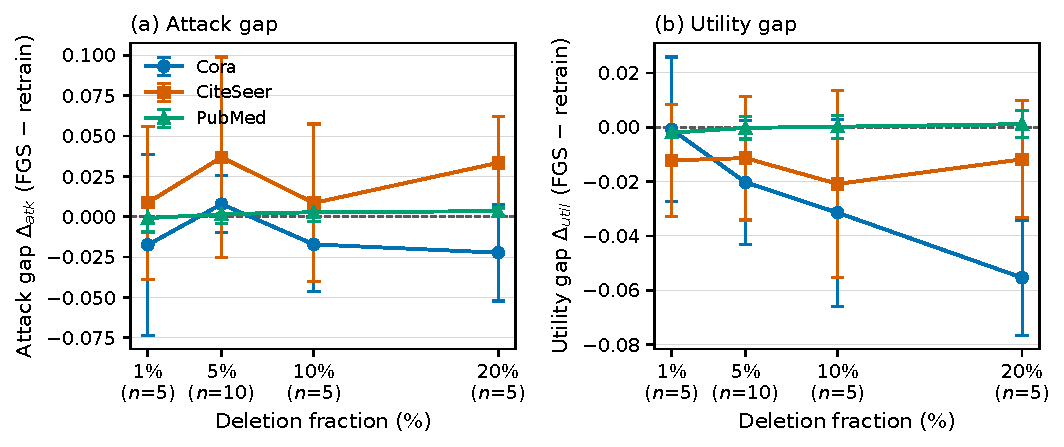
\includegraphics[width=0.92\textwidth]{Fig3.pdf}\caption{Attack gap (left) and utility gap (right) to retrain vs.\ deletion fraction (mean $\pm$ SD; 1\%/10\%/20\% at $n = 5$ seeds, 5\% at $n = 10$). PubMed is flat; Cora collapses at 20\%; CiteSeer is elevated at every fraction. Wilcoxon signed-rank p-values for the $n = 5$ comparisons are reported in the text.}\end{figure}

\begin{table}[htbp]\centering\small
\caption{Wall-clock time relative to retraining (median over the same 10 seeds as Table 4, single-machine re-run; 2 CPUs). Values $< 1$ mean faster than retraining. The fgs attack entry reports the median with its full range (seed variance is high for the 80-candidate rule); the other entries are medians. Timing was recorded for the attack-calibrated and hybrid variants on CiteSeer only (``---'' elsewhere). Timing basis per row group: the FGS and retrain-family rows (fgs (KS), GNNDelete, fgs attack) are total wall-clock medians on one host; the MEGU and ETR rows are procedure time excluding base-classifier training, as disclosed in Section 5, divided by the harness's recorded retrain seconds for the same seed; the fgs hybrid row is the end-to-end total (the KS trajectory plus its selection overhead).}
\begin{tabular}{lccc}\toprule Method & Cora & CiteSeer & PubMed\\\midrule
fgs (KS) & 0.35$\times$ & 0.31$\times$ & 0.30$\times$\\
GNNDelete & 0.20$\times$ & 0.22$\times$ & 0.19$\times$\\
MEGU & 0.068$\times$ & 0.052$\times$ & 0.045$\times$\\
ETR & 0.014$\times$ & 0.008$\times$ & 0.011$\times$\\
fgs attack (attack-calibrated run) & --- & 0.63$\times$ (range 0.49--0.74$\times$) & ---\\
fgs hybrid (total) & --- & 0.32$\times$ & ---\\\bottomrule
\end{tabular}\end{table}

The wide range on the attack-calibrated row is seed variance (different seeds settle on different candidates), not uncertainty about the method itself. Timing ratios are hardware-dependent: the ranges above were measured on 2 CPUs with no GPU, and the absolute seconds will shift on different hardware, though the relative ordering of the methods is stable.

\subsection{Diagnostics: when the KS proxy diverges}
Figure 4 shows the per-iterate KS, attack, and utility trajectories for one configuration per dataset, with the KS-selected and attack-optimal iterates marked. We diagnose the proxy/optimum mismatch systematically, not from a single seed: across all 30 configurations (the dataset--seed pairs of the main sweep) we correlate the KS-minimum iterate with the attack-optimal iterate (minimizing $|$attack $-$ retrain$|$). On CiteSeer the two are uncorrelated (Pearson $r = 0.05$, $p = 0.89$; Spearman $r = -0.00$, $p = 0.99$; mean absolute step difference 8.8)---the KS proxy shows essentially no detectable association with where the attack optimum lies across configurations. On Cora, they track each other (Pearson $r = 0.62$, $p = 0.058$; Spearman $r = 0.59$, $p = 0.070$; mean $|\Delta| = 4.7$ steps), and on PubMed the relationship is weak (Pearson $r = 0.44$, $p = 0.20$; mean $|\Delta| = 9.4$ steps, inflated by seeds where the KS minimum sits at step 0). Pooling across datasets would mix these heterogeneous regimes (CiteSeer $r = 0.05$, Cora $r = 0.62$, PubMed $r = 0.44$), so we report per-dataset values only. The CiteSeer seed-123 trajectories in Figure 4 (KS minimum at step 26, attack optimum at step 40, non-monotone KS) are thus one instance of a dataset-wide pattern, not an anecdote: on CiteSeer the stopping rule optimizes an objective uncorrelated with the attack metric. This proxy/optimum mismatch is our leading explanation for the CiteSeer weakness. (Signposting: the projection contrast is measured under both stopping rules---the fgs attack and fgs noproj-attack rows of Table 4 use the attack-calibrated rule, differing only in the projection, and the KS-stopped pair of Section 6.1 repeats the contrast under the non-circular rule, with the same conclusion.) The attack-calibrated rule exists precisely for this case, and the hybrid recovers about a third of its benefit at low cost. External results locate the weakness in the statistic as much as in this dataset. Aggregate distribution matching can mask per-sample deviations from retraining, which is why per-sample alignment targets have been proposed in its place \cite{sala2026}; and matching a never-trained proxy has identifiability limits, since for some facts no oracle-free threshold separates forgotten from never-learned \cite{distrestore2026}. Both readings fit what we observe: the KS minimum reports an aggregate match while the attack, a per-edge ranking, disagrees; and the shadow-retrain check in the Limitations shows the verdict moving when the reference changes. An alternative route predicts the retrained model's outputs directly and matches those, as datamodel matching does \cite{dmm2024}, at the price of an attribution model we do not have for link prediction.

\begin{figure}[htbp]\centering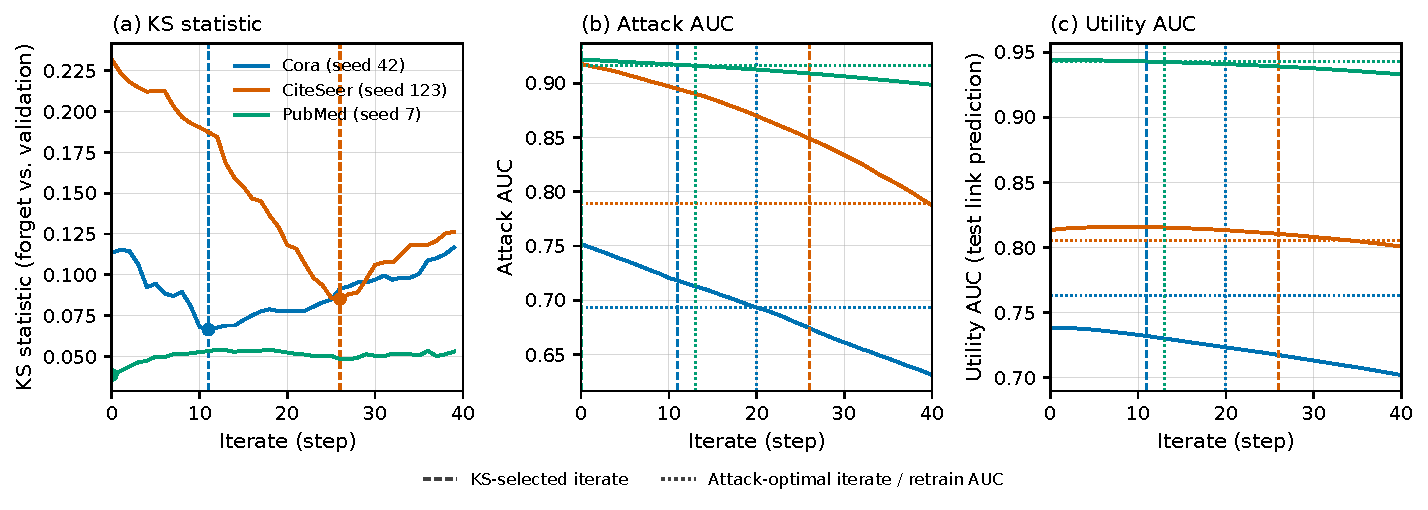
\includegraphics[width=0.92\textwidth]{Fig4.pdf}\caption{Per-iterate KS statistic, attack AUC, and utility AUC for one configuration per dataset (Cora seed 42, CiteSeer seed 123, PubMed seed 7). Dashed: KS-selected iterate; dotted: attack-optimal iterate (minimizing $|$attack $-$ retrain$|$). On CiteSeer seed 123, the two diverge (26 vs 40), diagnosing the proxy/optimum mismatch; on PubMed seed 7 the KS minimum is at step 0.}\end{figure}

\subsection{GraphSAGE transfer: a smoke test, not evidence}
We ran FGS (KS stopping) on a GraphSAGE backbone for Cora seed 42: attack gap +0.046 and utility gap +0.037 relative to the GraphSAGE retrain, at 0.48$\times$ retraining time---qualitatively similar to the GCN behavior (small positive attack gap, preserved utility, 2$\times$ speedup). A second configuration timed out on our 2-CPU hardware. With $n = 1$, this is a smoke test that the formulation is not GCN-specific, not a generalization claim; we state it as such.

\subsection{Fixed-step ablation: does adaptive stopping help?}
We compare the KS-selected iterate against fixed stopping schedules (steps 0, 10, 20, 30, 40) on all 30 configurations, using paired differences of the attack gap to retrain (Table 8). KS-adaptive stopping beats fixed short schedules (steps 0 and 10) and fixed long schedules (steps 30 and 40) decisively (all $p < 0.001$, $|d_z| > 1.0$): stopping too early under-forgets, stopping too late over-forgets. However, fixed step 20 is statistically tied with KS-adaptive stopping (paired attack-gap difference $-0.0001$, $p = 0.97$; utility difference +0.0004, $p = 0.67$)---a confirmed tie rather than an absence of evidence: the pooled interval is tightly centered on zero, and the per-dataset split below shows no detectable difference on any dataset either. This comparison pools all 30 configurations across the three datasets, mixing the heterogeneous per-dataset regimes diagnosed in Section 6.4. Read the tie as an aggregate statement; the per-dataset split follows. Per dataset (the pooled comparison of Table 8 split by dataset, recomputed from the archived trajectories), the step-20 attack differences are +0.009 on Cora ($p = 0.27$), $-0.008$ on CiteSeer ($p = 0.29$), and $-0.001$ on PubMed ($p = 0.74$)---no per-dataset loss or win is detectable either.

\begin{table}[htbp]\centering\small
\caption{KS-adaptive vs.\ fixed-step stopping, $n = 30$ configs: paired difference (KS-selected gap minus fixed-step gap) with two-sided t-test. Negative attack difference means KS is closer to retrain.}
\begin{tabular}{lcccc}\toprule Fixed step & Attack $\Delta$ & $p$ & Utility $\Delta$ & $p$\\\midrule
0 & $-0.042$ & $< 0.001$ & $-0.006$ & $< 0.001$\\
10 & $-0.024$ & $< 0.001$ & $-0.005$ & $< 0.001$\\
20 & $-0.0001$ & 0.97 & +0.0004 & 0.67\\
30 & +0.027 & $< 0.001$ & +0.007 & $< 0.001$\\
40 & +0.056 & $< 0.001$ & +0.015 & $< 0.001$\\\bottomrule
\end{tabular}\end{table}

The data support a weaker conclusion than ``adaptive dominates any fixed schedule''. KS stopping is competitive with the best fixed schedule without requiring tuning. It strictly dominates the fixed schedules one would naively choose (too few or too many steps). The obvious objection (``if step 20 ties, why the machinery?'') has a direct answer: step 20 was found by looking at the answer. It is close to the median of the KS-selected steps on these three graphs, but the per-seed KS selections span 9--29 steps on Cora, 13--28 on CiteSeer, and 0--39 on PubMed---on PubMed seed 7 the right answer is literally zero steps, on others nearly forty. A fixed step chosen without this knowledge risks exactly the failure modes the table shows: stop too early and you under-forget, too late and you over-forget, both decisively worse than the adaptive rule (all $p < 0.001$). What the KS rule buys is per-dataset robustness without a tuned constant. It lands near the per-configuration optimum with no labeled sweep to find it, and it adapts where a fixed schedule cannot (e.g., the PubMed step-0 cases).

\section{Discussion: the forgetting--utility--efficiency frontier}
Across the sweep, the evidence is a three-way tradeoff among forgetting, utility, and efficiency, with the ranking depending on the dataset, the deletion fraction, and the stopping rule. Every reading in this section is conditional on the tested regime, as scoped in the Limitations, and does not extend beyond it. Plain KS stopping is the fastest FGS variant: near-retrain on PubMed at all tested fractions and on Cora at small fractions, at 0.30--0.35$\times$ retraining time (median), but it degrades at 20\% on Cora and shows the largest attack gaps on CiteSeer. The decomposition of Section 6.1 sits underneath the whole frontier: the ascent forgets, the projection protects utility, and the stopping rule trades the two against cost---so the frontier is over components as much as over methods. No single method dominates all three axes. (MEGU and ETR stay off this frontier: descriptive rows only, under the encoder caveat of Section 5, though their procedure times are the lowest recorded of any single method, Table 7.) GNNDelete (our NumPy port, validated on PubMed and unvalidated on Cora and CiteSeer) runs at median 0.19--0.22$\times$ vs.\ 0.30--0.35$\times$ retraining time for KS-stopped FGS; tuned on held-out seeds it is the faster procedure with comparable utility, FGS holds the smaller absolute attack gap on Cora and PubMed, and CiteSeer is a tie on absolute gap with the signed gap favoring the tuned baseline (Section 6.1); at the untuned port setting it forgets less well on Cora/CiteSeer and over-forgets on PubMed. Fine-tuning does not forget, NegGrad destroys utility, and unlinking alone (UtU) does not reach retrain indistinguishability. Attack-calibrated stopping is the thorough option: it closes the CiteSeer gap under the evaluation auditor---but only under that auditor. A shadow-retrain stopping check reopens it (+0.060 vs.\ +0.008); the shadow stop is itself unstable per seed, sitting on a flat KS curve, and re-computation from the archived trajectories brackets the shadow gap at +0.051 to +0.060, with the conclusion unchanged (the Limitations give the full reading). The cost is 0.49--0.74$\times$ retraining (median 0.63$\times$), sacrificing most of the speed advantage, and it over-forgets on PubMed. The hybrid is the compromise: a significant but partial share of the calibration gain (about a third of the KS-to-attack mean improvement) at near-KS cost. That is the frontier: no configuration dominates all three axes.

\textbf{Why CiteSeer is hard.} The diagnostics point to a proxy/optimum mismatch: across all ten CiteSeer seeds, the KS-minimum iterate is uncorrelated with the attack-optimal iterate ($r = 0.05$), while the two track each other on Cora ($r = 0.62$) and relate only weakly on PubMed ($r = 0.44$). The CiteSeer attack-gap mean (+0.037 $\pm$ 0.062) also deserves a robustness caveat: the median is +0.018, and a single seed (7777, gap +0.181---roughly 3$\times$ the next-largest value) drives the mean and most of the variance. Leave-one-out, dropping seed 7777 moves the mean to +0.021 (SD 0.038); dropping any other seed leaves the mean between +0.032 and +0.046. Notably, seed 7777 is also the worst seed for GNNDelete (gap +0.173), so the draw is a hard one, not an FGS-specific artifact. The ``largest and most variable'' characterization of CiteSeer should therefore be read with this skew in mind: typical seeds sit near +0.02, with one anomalous draw pulling the mean up. A plausible mechanism for the underlying mismatch is CiteSeer's sparser, noisier graph structure, where the validation-edge score distribution is itself a poor stand-in for the retrained forget-edge distribution. We have not isolated the cause, so the mismatch stands as a diagnosis. Equivalence testing makes the same point from the other direction: CiteSeer is the one dataset whose attack gap is not equivalent to retraining at the $\pm$0.02 margin, and establishing equivalence there would need $\approx$85 seeds (Section 6.1).

\textbf{Why Cora collapses at 20\%.} At large deletion fractions, the forget set is a substantial part of the training graph; the projected trajectory must travel far, and the first-order protection of Proposition 1 degrades over many steps as the anchor $g_r$ itself moves. The observed utility drop of 0.05--0.06 ($p = 0.004$ at $n = 5$; Wilcoxon $p = 0.0625$) is suggestive of the expected failure mode of a local method pushed outside its local regime, but at $n = 5$ this is a hypothesis, not an established failure mode (Section 6.2); the accompanying attack gap ($-0.022$) is not distinguishable from zero at $n = 5$, so the supported claim is a utility collapse. We count it a limitation of the method; the evaluation only exposes it.

\textbf{Collateral damage and prevention versus repair.} The collateral-damage pattern FGS maps on citation graphs---an unlearning step whose damage spills onto retained, similar items---is recognized across domains: CRAGRU \cite{cragu2025} names the analogous ``unlearning bias'' in recommender unlearning, where deleting one user's data distorts recommendations for behaviorally similar users, and isolates the target's influence by retrieval rather than by a single-model projected update. The utility fragility that motivates FGS's projection has likewise been addressed from the opposite direction: Khan et al.\ \cite{khan2026} harden a GCN architecturally at training time (Fix-GCN) against adversarial perturbations of graph structure and node features; FGS works the other end of the timeline: it repairs an already-trained GCN post hoc, after legitimate, requested deletions. Prevention at training time, repair after it; the perturbation object is the same.

\section{Limitations}
\begin{enumerate}
\item \textbf{No certificate.} FGS is approximate and empirical; we offer no certified-unlearning guarantee, and the fixed non-adaptive auditor may miss residual signal.
\item \textbf{Scope.} Edge deletion only, on homophilic citation graphs, with GCN (plus one GraphSAGE smoke test). Node and feature deletion, heterophilic graphs, and larger backbones are untested.
\item \textbf{GNNDelete port fidelity.} The port is validated on PubMed and unvalidated on Cora and CiteSeer, for the reasons stated in Section 5: on PubMed the port's AUROC($E_d$) deltas fall inside Cheng et al.'s published range; on Cora the same statistic lands at the retrain level because this harness's retrain reference already separates deleted from remaining edges, leaving the statistic little headroom; CiteSeer is not among Cheng et al.'s datasets. The port remains an adaptation (deviations D1--D5), not the official implementation; substituting the official implementation was costed at 2--4 days of engineering and declined, because the result would still be an adaptation in the same respects. $\lambda$ is tuned per dataset on held-out seeds ($\lambda^\star = 1.0/0.5/4.0$), and the tuned head-to-head (Table 5) is the primary comparison. What remains open is the unvalidated status on two of three datasets, which attaches to the tuned CiteSeer tie and the Cora difference. The severe PubMed over-forget at $\lambda = 1.0$ ($-0.085$) is a port-setting artifact---at $\lambda^\star = 4.0$ it is $-0.014$---and no claim in this paper rests on it.
\item \textbf{Stopping is the weak link.} The KS proxy diverges from the attack optimum on CiteSeer; the attack-calibrated rule fixes this only by sacrificing the speed advantage and over-forgetting on PubMed. The KS-stopped no-projection ablation (Section 6.1) removes the confound that attaches to the attack-stopped comparison: the projection's utility contribution is demonstrated under the KS rule itself, not only under the circular attack-calibrated rule.
\item \textbf{Attack calibration is auditor-circular.} The fgs attack rule selects the iterate with the same link-inference auditor family used for evaluation (disjoint negatives, but the same scorer and attack). We tested a mild adaptive stopping calibration on the same 80-candidate trajectory that produced Table 4's fgs attack column: a per-seed shadow retrain, stopping at the iterate whose forget-edge scores best match the shadow retrain's (KS); the evaluation auditor and its scoring are unchanged---only the calibration of the stop changes. The attack-calibrated choice on this trajectory reproduces the Table 4 value exactly (CiteSeer gap +0.008 $\pm$ 0.070), so the comparison is on identical configurations. The shadow-calibrated stop (median stop 17, against an attack-calibrated median stop of 30; per-seed shadow-selected steps are in the reproduction package) does not reproduce the attack-calibrated gap closure: its CiteSeer attack gaps are +0.060 $\pm$ 0.050 (paired difference +0.052, $p = 0.003$, $d_z = 1.27$, $n = 10$)---essentially the plain-KS level. The CiteSeer gap closure should therefore be read as ``indistinguishable under this auditor,'' not as auditor-independent forgetting. The shadow stop itself is unstable at the per-seed level. The selection rule is the earliest iterate minimizing the KS distance between the iterate's forget-edge scores and the shadow retrain's; that distance curve is flat near its minimum, so floating-point-level variation in the shadow retrain across recomputations (runs under differing thread counts) moves the argmin among near-tied iterates, and re-computation brackets the reported shadow gap (+0.051 to +0.060 across recomputations) with the paired difference significant in both computations; the conclusion---the shadow-calibrated stop does not reproduce the closure---is unchanged.
\item \textbf{Large fractions.} Utility appears to degrade at 20\% deletion on Cora ($n = 5$, exploratory---see Section 6.2); treat FGS as a small-deletion tool pending confirmation at larger $n$.
\item \textbf{Absolute attack AUC stays high.} ``Forgotten'' means indistinguishable from retraining, not unpredictable---the graph itself leaks link information.
\item \textbf{Compute.} All experiments ran on 2 CPUs without a GPU; timings are hardware-specific, though relative comparisons hold.
\item \textbf{MEGU/ETR base-model mismatch.} The two rows are computed from node-classifier encoders never trained on edges (the governing caveat of the setup section). Absolute AUCs are not like-for-like with the link-prediction baselines, and the gaps against the FGS retrain reference conflate unlearning behavior with classifier-embeddings-as-link-features. The over-forgetting direction is consistent across 30/30 (MEGU) and 26/30 (ETR) seeds; the magnitudes are the part to read cautiously.
\item \textbf{Equivalence is dataset-bound.} Equivalence to retraining is established only on PubMed and Cora, at the $\pm$0.02 margin and $n = 10$. On CiteSeer it is not establishable at feasible seed counts ($\approx$85 seeds at the observed variance), so CiteSeer's standing in this study is ``not shown equivalent'' at this design's scale, in either direction.
\end{enumerate}

\section{Future Work}
The primary open problem is a stopping rule that inherits the KS rule's cost and the attack rule's calibration---the hybrid is a first step, but a principled proxy (e.g., a distributional distance weighted by the attack's ranking geometry) could close the gap. Second, stronger membership-inference auditors: evaluating FGS against adaptive, shadow-model adversaries beyond the shadow-retrain stopping check of Limitation 5 would test whether the retrain gap survives a stronger adversary. Third, node and feature deletion, where the blast-radius analysis suggests the surgery should apply, but the forget gradient needs re-derivation. Finally, the CiteSeer proxy/optimum mismatch deserves a mechanistic explanation, and CiteSeer-scale equivalence deserves a powered design: on the order of 85 seeds at the observed variance, or a lower-variance auditor, would close the one equivalence question this study leaves open.

\section{Reproducibility Statement}
All experiments use public datasets (Cora, CiteSeer, PubMed) with the splits and seeds documented in Section 5. The experiment code, raw per-seed JSON outputs, and analysis scripts are archived with the submission; every aggregate in this paper is recomputed from the raw JSON by the analysis script, and the audit trail (claim-by-claim recomputation) is included as supplementary material. The archive also includes the verification scripts used here: scripts/full\_rerun.py (frozen-pipeline re-run establishing seed-pooling exchangeability and same-machine timings), scripts/compute\_utu.py (unlink-only baseline), and scripts/shadow\_auditor.py (shadow-retrain auditor test). The verification experiments---GNNDelete validation against Cheng et al.'s published numbers, the held-out $\lambda$ tuning and tuned head-to-head, the KS-stopped no-projection ablation, the TOST equivalence tests, and the Benjamini--Hochberg/Bonferroni corrections---are archived with their run log and per-unit outputs (fix-round-test40/), and every number they contribute to Sections 5--8 is recomputed from those outputs.

\appendix
\section{Per-seed tables}
\begin{table}[htbp]\centering\scriptsize
\caption{Per-seed FGS (KS) gaps to retrain, 5\% deletion.}
\begin{tabular}{llrrrr}\toprule Dataset & Seed & $\Delta_{atk}$ & $\Delta_{util}$ & FGS time (s) & Retrain time (s)\\\midrule
citeseer & 7 & +0.0526 & -0.0340 & 45.3 & 117.9\\
citeseer & 42 & -0.0053 & +0.0170 & 44.7 & 116.2\\
citeseer & 123 & +0.0629 & +0.0046 & 45.3 & 115.0\\
citeseer & 999 & +0.0061 & -0.0330 & 118.6 & 230.3\\
citeseer & 2024 & +0.0188 & -0.0010 & 84.6 & 190.0\\
citeseer & 2025 & -0.0431 & -0.0522 & 73.8 & 233.0\\
citeseer & 5555 & +0.0795 & -0.0218 & 97.6 & 329.2\\
citeseer & 7777 & +0.1807 & +0.0135 & 110.5 & 242.0\\
citeseer & 31337 & -0.0019 & -0.0028 & 54.2 & 136.3\\
citeseer & 31338 & +0.0178 & -0.0039 & 86.9 & 212.2\\
cora & 7 & +0.0035 & -0.0273 & 14.1 & 36.0\\
cora & 42 & +0.0229 & -0.0320 & 14.7 & 37.0\\
cora & 123 & +0.0220 & +0.0274 & 13.9 & 37.2\\
cora & 999 & -0.0045 & -0.0078 & 33.4 & 76.4\\
cora & 2024 & +0.0043 & -0.0001 & 15.3 & 41.5\\
cora & 2025 & -0.0255 & -0.0329 & 26.9 & 62.4\\
cora & 5555 & +0.0267 & -0.0370 & 28.2 & 63.6\\
cora & 7777 & -0.0037 & -0.0305 & 49.7 & 104.2\\
cora & 31337 & +0.0302 & -0.0520 & 15.8 & 44.7\\
cora & 31338 & +0.0021 & -0.0108 & 27.1 & 69.9\\
pubmed & 7 & +0.0058 & +0.0018 & 34.3 & 90.9\\
pubmed & 42 & -0.0008 & -0.0021 & 46.1 & 127.9\\
pubmed & 123 & -0.0028 & -0.0077 & 33.7 & 89.5\\
pubmed & 999 & +0.0033 & -0.0010 & 117.2 & 316.6\\
pubmed & 2024 & +0.0049 & +0.0035 & 54.9 & 142.6\\
pubmed & 2025 & -0.0027 & -0.0038 & 85.8 & 226.5\\
pubmed & 5555 & -0.0090 & -0.0012 & 66.6 & 190.8\\
pubmed & 7777 & +0.0116 & +0.0069 & 116.6 & 323.6\\
pubmed & 31337 & +0.0018 & -0.0011 & 54.4 & 146.9\\
pubmed & 31338 & +0.0037 & +0.0023 & 77.5 & 225.7\\\bottomrule
\end{tabular}\end{table}

\section{Stopping-rule trajectories}
Per-iterate KS, attack, and utility trajectories for the three diagnostic configurations are plotted in Figure 4; the underlying arrays (the attack and utility arrays hold 41 values each; the KS array holds 40 values, steps 0--39, because the KS statistic is computed inside the 40-step loop) are archived in results/fixedstep.json under configs (keys ks, attack, util) with per-config provenance (cache file, JSON file, and RNG streams).

\section{Claim-by-claim audit trail}
The headline quantitative claims in Sections 6.1--6.6 are checked against the raw per-seed JSONs (reproduction-package/results/per\_seed/*.json) by the verifier reproduction-package/scripts/verify\_reproduction.py, which recomputes every headline number from the raw outputs and exits nonzero on any mismatch; expected values are pinned in reproduction-package/expected/headline\_numbers.json. The fixed-step validation (maximum attack deviation 0.0059 vs.\ tolerance 0.01) is recorded in reproduction-package/results/fixedstep.json under validation.

\section*{Declarations}
\textbf{Funding.} No funds, grants, or other support was received.

\textbf{Competing interests.} The author has no relevant financial or non-financial interests to disclose.

\textbf{Ethics approval.} Not applicable.

\textbf{Consent to participate.} Not applicable.

\textbf{Consent for publication.} Not applicable.

\textbf{Data availability.} The Planetoid Cora, CiteSeer and PubMed datasets are publicly available via PyTorch Geometric \cite{planetoid2016}; the generated per-seed result data are included in the reproduction package submitted as supplementary material; a public repository will be released on acceptance.

\textbf{Materials availability.} Not applicable.

\textbf{Code availability.} The experiment code, baseline adapters, and analysis scripts are in the same supplementary reproduction package; a public release will follow on acceptance.

\textbf{Author contributions.} The author conceived and designed the study, performed the experiments and analysis, and wrote and approved the manuscript.

\bibliography{refs}
\end{document}
